\documentclass[10pt,a4paper]{article}
\usepackage[margin=1.8cm,top=1.6cm,bottom=1.7cm]{geometry}
\usepackage{amsmath,amssymb,booktabs,graphicx,float,xcolor,tikz,caption,enumitem,array,multirow,tabularx,microtype,url}
\usepackage[hidelinks]{hyperref}
\microtypesetup{expansion=false}
\usetikzlibrary{arrows.meta,positioning,fit,backgrounds,calc}
\captionsetup{font=small,labelfont=bf,skip=3pt}
\setlength{\parindent}{0pt}\setlength{\parskip}{3pt}
\newcommand{\studentname}{Huzaifa Abid}
\newcommand{\studentid}{25280009}
\newcommand{\repourl}{https://github.com/ihuzafaone/DLSTG-PA2}
\newcommand{\Q}[2]{\par\smallskip\noindent\textbf{#1}\ #2\par}
\begin{document}
\begin{center}
{\large\textbf{AI651 -- Deep Learning for Space, Time and Graphs \; Assignment 2}}\\[2pt]
\studentname\ (\studentid) \quad Fall 2026\\[2pt]
\textbf{Code (public GitHub repository):} \url{\repourl}
\end{center}
\graphicspath{{../figures/}}
% ============================================================== QUESTION 1
\section*{Question 1 --- River Forecasting Proposal}
\addcontentsline{toc}{section}{Question 1 --- River Forecasting Proposal}

\noindent\textbf{Proposal in one paragraph.} Every 10 minutes we forecast the water level $60$ minutes ahead at S1--S4 (with the intermediate $10,\dots,50$-minute levels and an 80\,\% interval) using a \emph{river-graph forecaster}: per-station causal temporal encoders, followed by \emph{lag-aware attention} that lets every station read only its physically plausible upstream sources (reservoir releases, upstream stations, the monitored tributary T1, rainfall) at the lag implied by a flow-dependent travel time. The unmonitored tributary is a latent node driven by R2 rainfall, and the announced release schedule enters as known future tokens. The system is small ($\approx\!1.7\times10^{5}$ parameters, a few milliseconds per forecast) and is built to keep working with missing, late or contradictory data.

% ------------------------------------------------------------------ 1
\subsection*{1.\ Architecture diagram}
\begin{figure}[H]
\centering
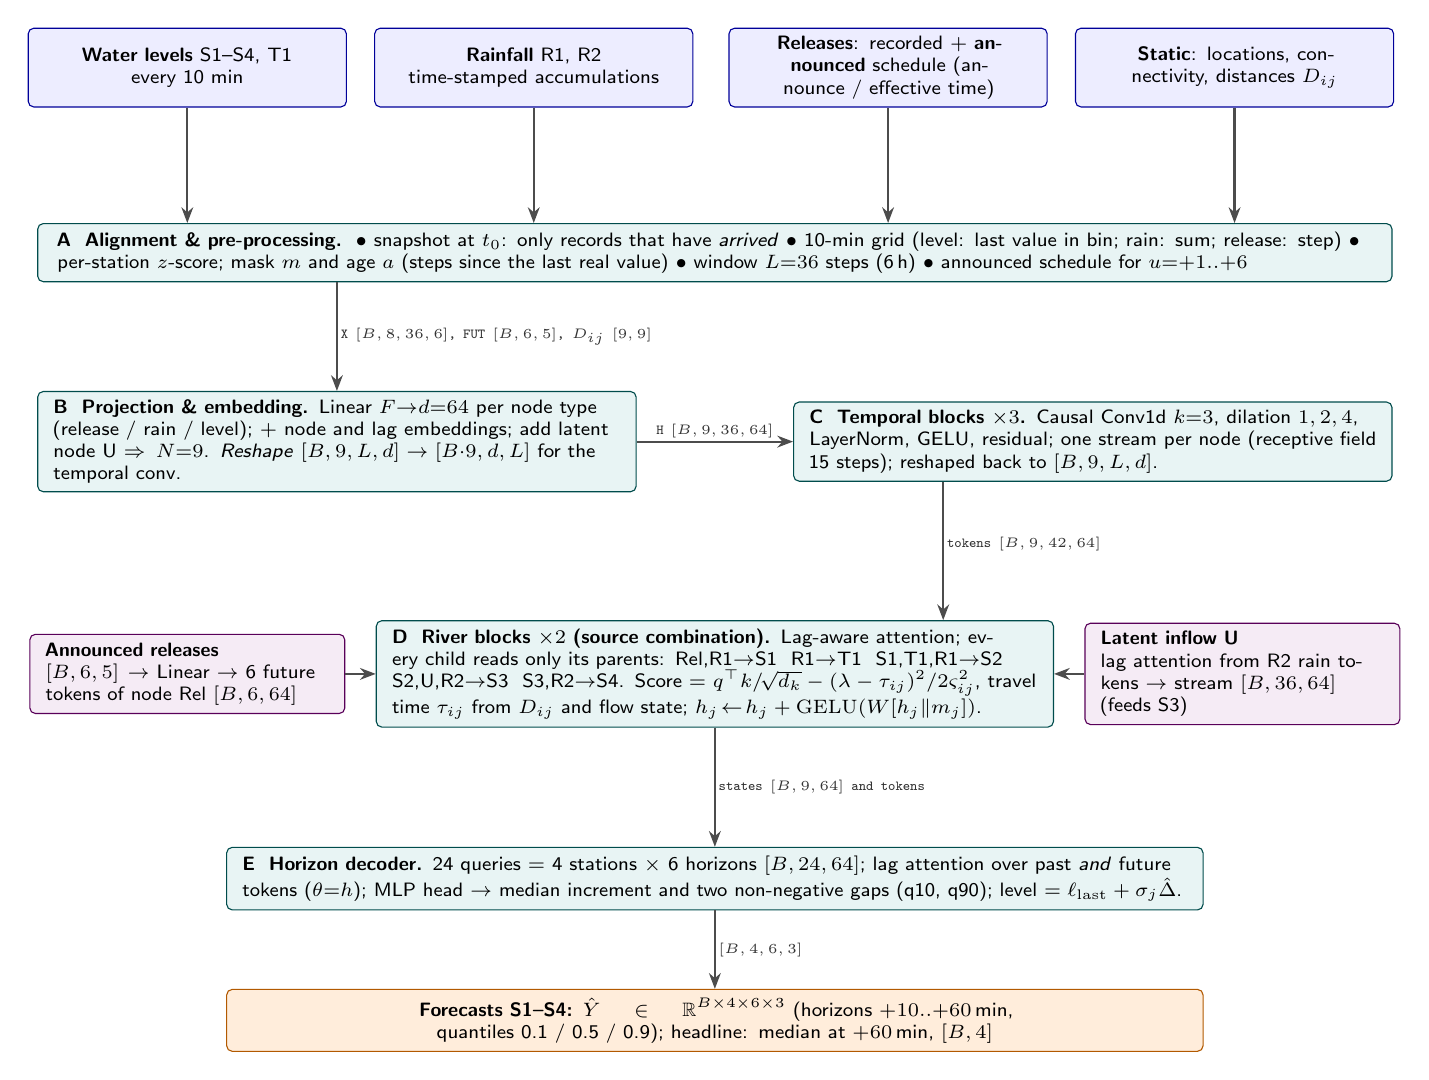
\begin{tikzpicture}[
  font=\sffamily\scriptsize, x=1cm, y=1cm,
  nsrc/.style={draw=blue!60!black,rounded corners=2pt,fill=blue!7,minimum width=40mm,minimum height=10mm,inner sep=2pt,align=center,text width=39mm},
  nblk/.style={draw=teal!60!black,rounded corners=2pt,fill=teal!9,inner sep=3pt,align=left},
  nside/.style={draw=violet!70!black,rounded corners=2pt,fill=violet!8,inner sep=3pt,align=left},
  nout/.style={draw=orange!70!black,rounded corners=2pt,fill=orange!14,inner sep=3pt,align=center},
  arr/.style={-{Stealth[length=2mm]},thick,gray!60!black},
  ndim/.style={font=\tiny\ttfamily,fill=white,inner sep=1pt,text=black!80}]
% sources
\node[nsrc] (s1) at (2.0,0)  {\textbf{Water levels} S1--S4, T1\\ every 10 min};
\node[nsrc] (s2) at (6.4,0)  {\textbf{Rainfall} R1, R2\\ time-stamped accumulations};
\node[nsrc] (s3) at (10.9,0) {\textbf{Releases}: recorded $+$ \textbf{announced} schedule (announce / effective time)};
\node[nsrc] (s4) at (15.3,0) {\textbf{Static}: locations, connectivity, distances $D_{ij}$};
% A
\node[nblk,text width=167mm,minimum width=172mm] (A) at (8.7,-2.35) {\textbf{A\ \ Alignment \& pre-processing.}\ \ $\bullet$ snapshot at $t_0$: only records that have \emph{arrived} $\bullet$ 10-min grid (level: last value in bin; rain: sum; release: step) $\bullet$ per-station $z$-score; mask $m$ and age $a$ (steps since the last real value) $\bullet$ window $L{=}36$ steps (6\,h) $\bullet$ announced schedule for $u{=}{+}1..{+}6$};
% B, C
\node[nblk,text width=72mm,minimum width=76mm] (B) at (3.9,-4.75) {\textbf{B\ \ Projection \& embedding.} Linear $F{\to}d{=}64$ per node type (release / rain / level); $+$ node and lag embeddings; add latent node U $\Rightarrow N{=}9$. \emph{Reshape} $[B,9,L,d]\!\to\![B{\cdot}9,d,L]$ for the temporal conv.};
\node[nblk,text width=72mm,minimum width=76mm] (C) at (13.5,-4.75) {\textbf{C\ \ Temporal blocks $\times3$.} Causal Conv1d $k{=}3$, dilation $1,2,4$, LayerNorm, GELU, residual; one stream per node (receptive field 15 steps); reshaped back to $[B,9,L,d]$.};
% D with side inputs
\node[nblk,text width=82mm,minimum width=86mm] (D) at (8.7,-7.7) {\textbf{D\ \ River blocks $\times2$ (source combination).} Lag-aware attention; every child reads only its parents: Rel,R1$\to$S1\ \ R1$\to$T1\ \ S1,T1,R1$\to$S2\ \ S2,U,R2$\to$S3\ \ S3,R2$\to$S4. Score $=q^{\top}k/\!\sqrt{d_k}-(\lambda-\tau_{ij})^{2}/2\varsigma_{ij}^{2}$, travel time $\tau_{ij}$ from $D_{ij}$ and flow state; $h_j\!\leftarrow\!h_j+\mathrm{GELU}(W[h_j\Vert m_j])$.};
\node[nside,text width=36mm,minimum width=40mm] (F) at (2.0,-7.7) {\textbf{Announced releases}\\ $[B,6,5]\to$ Linear $\to$ 6 future tokens of node Rel $[B,6,64]$};
\node[nside,text width=36mm,minimum width=40mm] (U) at (15.4,-7.7) {\textbf{Latent inflow U}\\ lag attention from R2 rain tokens $\to$ stream $[B,36,64]$ (feeds S3)};
% E, output
\node[nblk,text width=120mm,minimum width=124mm] (E) at (8.7,-10.3) {\textbf{E\ \ Horizon decoder.} 24 queries $=$ 4 stations $\times$ 6 horizons $[B,24,64]$; lag attention over past \emph{and} future tokens ($\theta{=}h$); MLP head $\to$ median increment and two non-negative gaps (q10, q90); level $=\ell_{\rm last}+\sigma_j\hat\Delta$.};
\node[nout,text width=120mm,minimum width=124mm] (O) at (8.7,-12.1) {\textbf{Forecasts S1--S4:} $\hat Y\in\mathbb{R}^{B\times4\times6\times3}$ (horizons $+10..{+}60$\,min, quantiles 0.1 / 0.5 / 0.9);\ headline: median at $+60$\,min, $[B,4]$};
% arrows
\foreach \i in {s1,s2,s3,s4} \draw[arr] (\i.south) -- (\i.south |- A.north);
\draw[arr] (A.south -| B.north) -- node[ndim,right]{X $[B,8,36,6]$,\ FUT $[B,6,5]$,\ $D_{ij}$ $[9,9]$} (B.north);
\draw[arr] (B.east) -- node[ndim,above]{H $[B,9,36,64]$} (C.west);
\coordinate (cx) at (11.6,0);
\draw[arr] (cx |- C.south) -- node[ndim,right,pos=0.45]{tokens $[B,9,42,64]$} (cx |- D.north);
\draw[arr] (F.east) -- (D.west);
\draw[arr] (U.west) -- (D.east);
\draw[arr] (D.south) -- node[ndim,right]{states $[B,9,64]$ and tokens} (E.north);
\draw[arr] (E.south) -- node[ndim,right]{$[B,4,6,3]$} (O.north);
\end{tikzpicture}
\caption*{\textbf{Figure Q1.} Architecture. $B$ = batch axis (independent issuance times; $B{=}1$ in operation); $L{=}36$ past steps; $N{=}9$ nodes (Rel, R1, R2, T1, S1, S2, U, S3, S4); token axis $42=36$ past $+\,6$ future steps; $d{=}64$. \emph{Alignment} puts all stations on one clock but does not remove the physical delay between stations (modelled explicitly in D and E); \emph{projection} maps each node type's features to the shared width $d$; \emph{reshapes} are noted on the blocks. Training: weighted pinball loss on observed targets $+$ celerity prior, chronological split, node/gap dropout and simulated delays.}
\end{figure}

% ------------------------------------------------------------------ 2
\subsection*{2.\ Assumptions}
\noindent\textbf{Supplied facts (not assumptions).} Four main-river stations S1$\to$S4 in flow order; reservoir above S1; monitored tributary T1 joins between S1 and S2; an \emph{unmonitored} tributary joins between S2 and S3; rain gauges R1, R2 with known locations; levels at S1--S4, T1 every 10\,min; rainfall with timestamps; recorded releases plus future schedules announced before each forecast (announcement and effective times); distances along the river; uneven spacing; travel times may change with conditions. \emph{Not supplied:} travel times, unmonitored inflow, future rain or levels, reporting delays, gauge quality.

\begin{table}[H]\centering\footnotesize
\renewcommand{\arraystretch}{1.12}
\begin{tabularx}{\linewidth}{@{}l>{\raggedright\arraybackslash}p{4.6cm}>{\raggedright\arraybackslash}X>{\raggedright\arraybackslash}X@{}}
\toprule
 & Assumption & Why reasonable & Effect on the design \\ \midrule
A1 & Records carry a measurement time stamp within $\pm1$ step of the 10-min grid.& Telemetry loggers are clock-driven; jitter of a minute or two is typical.& Re-gridding in block A (last value per bin; rain \emph{summed} per bin).\\
A2 & Levels are stage in metres on a fixed datum per gauge ($\approx\pm$1--2\,cm); rain gauges give accumulations (tipping bucket, $\approx0.2$\,mm).& Standard instrumentation; datum offsets between stations do not matter for forecasting changes.& Per-station standardisation $\mu_i,\sigma_i$; forecasts are \emph{increments} on the last observed level.\\
A3 & Arrival delay is usually $0$--$2$ steps, occasionally up to 1\,h; each record has a measurement and an arrival time.& Cellular/radio links are late rather than wrong; telemetry logs normally hold both stamps.& As-of snapshot at $t_0$; delays simulated in training (\S5).\\
A4 & Gaps are mostly short (1--6 steps) with rare long outages; spikes/flat-lines can be flagged by simple QC; failures are more likely during storms.& Usual sensor/communication behaviour; storms damage gauges.& Mask + age channels; node and gap dropout in training; QC-flagged values are treated as missing.\\
A5 & Several years of history are available, with multiple flood rises and release events, and a stable gate-operation regime.& A forecasting service is commissioned from an operating record; ``historical'' implies years, not days.& Modest model size ($\approx$0.17\,M parameters) and shared weights; chronological split; event oversampling.\\
A6 & Dominant flow is one-dimensional downstream; a disturbance moves at a celerity $c$ of order $1$--$3$\,m/s ($\approx4$--$11$\,km/h) that \emph{rises with stage}; no tide, no backwater from S4's bridge.& Kinematic/diffusive-wave behaviour of mountain rivers; the supplied map shows a free-flowing river.& \emph{Directed} graph (no downstream$\to$upstream links); causal lags $\lambda\!\ge\!0$; lag window $\le18$ steps (3\,h) inside $L{=}36$.\\
A7 & Travel times and attenuation depend on flow state; the 60-min horizon is comparable to travel time between neighbouring stations.& Celerity grows with depth; the horizon was chosen by the authority for this river.& Travel time $\tau_{ij}$ is \emph{state dependent} with a distance-based prior; spread $\varsigma_{ij}$ grows with distance.\\
A8 & The unmonitored tributary is mostly rain driven (R2 catchment, lag 1--3\,h), unregulated; its inflow shows up as a rise at S3 not explained by S2.& It lies between S2 and S3, below the reservoir, and has no gauge or control.& Latent node U fed by R2 rain tokens; S3/S4 decoders also see their own recent trend (it reveals inflow once it arrives).\\
A9 & Point rainfall at R1/R2 is a usable proxy of its sub-catchment's rain; antecedent 24\,h/72\,h rainfall indicates wetness.& Only two gauges exist; antecedent precipitation is the standard wetness proxy.& Rain nodes R1, R2 with learned lag kernels; antecedent sums as channels; widened intervals (\S6).\\
A10 & Announced schedules cover at least the next 60\,min; the dam$\to$S1 travel time is $<1$\,h; actual release usually follows the schedule within $\approx10\%$ and a step.& A schedule is announced to be acted on; S1 is the first station below the dam.& Future-release tokens on node Rel with \emph{effective} times; deviation channel; fallback in \S5(iv).\\
A11 & Channel and gate rules change slowly (months).& Typical for engineered rivers; abrupt changes would be communicated.& Scheduled retraining, drift monitor (\S5).\\
A12 & Flood-warning levels exist per station; forecasts support human decisions.& Standard in flood preparedness; output is advice, not automatic gate control.& Flood-weighted loss, quantile (interval) outputs.\\ \bottomrule
\end{tabularx}
\end{table}

% ------------------------------------------------------------------ 3
\subsection*{3.\ Forecasting task and data specification}
\noindent\textbf{Task.} Issuance time $t_0$ is any instant on the 10-min grid ($t_0=10k$ min); a forecast uses only records with arrival time $\le t_0$ (plus the schedule announced by then). \textbf{History window:} $L{=}36$ steps, $s\in\{-35,\dots,0\}$, i.e.\ $t_0-350,\dots,t_0$ min (6\,h; covers the assumed $\le3$\,h travel plus rainfall response). \textbf{Horizon:} $H{=}6$ steps, $h\in\{1,\dots,6\}$ = $t_0{+}10h$ min; the \emph{service output} is the level at $t_0{+}60$\,min ($h{=}6$) at S1--S4, the other horizons give the trajectory and training signal. \textbf{Output:} $\hat Y\in\mathbb{R}^{B\times4\times6\times3}$ (stations $\times$ horizons $\times$ quantiles $0.1/0.5/0.9$) converted to metres; $B$ is the batch axis of independent issuance times.

\begin{table}[H]\centering\scriptsize
\renewcommand{\arraystretch}{1.1}
\begin{tabularx}{\linewidth}{@{}>{\raggedright\arraybackslash}p{2.35cm}>{\raggedright\arraybackslash}p{2.9cm}>{\raggedright\arraybackslash}p{4.05cm}>{\raggedright\arraybackslash}X@{}}
\toprule
Input / output & Shape & Axes (channels) & Time coverage and availability at $t_0$ \\ \midrule
Levels S1--S4, T1 & $[B,5,36,6]$ & batch, station, step, channels: $z$-level, $\Delta z$ (10\,min), $z_s{-}z_{s-6}$ (1\,h trend), mask $m$, age $a$, QC flag & $t_0{-}350..t_0$ min at 10-min steps; latest value may be missing/late. Future levels \emph{not} available.\\
Rainfall R1, R2 & $[B,2,36,6]$ & batch, gauge, step, ch.: $\log(1{+}r)$, 1-h sum, 24-h and 72-h antecedent sums, $m$, $a$ & Same grid; accumulations over each 10-min bin (timestamps snapped). Future rain \emph{not} available.\\
Recorded releases & $[B,1,36,6]$ & batch, node Rel, step, ch.: actual $z$-release, schedule \emph{as issued then}, deviation, $\Delta$, $m$, $a$ & Same grid; actual release known up to $t_0$ (may lag).\\
Announced future releases & $[B,6,5]$ & batch, future step $u{=}1..6$, ch.: scheduled release, change vs.\ previous announcement, announcement age, lead $u/6$, mask & Effective times $t_0{+}10u$ min; announced at or before $t_0$. Pad/mask if the schedule is shorter.\\
Static graph data & $[9,9]$, $[9]$ (no batch axis) & distances $D_{ij}$ (km), parent mask $A_{ji}$, node-type id & Supplied (locations, connectivity, distances).\\
Node tensor $X$ (stack of the first three rows) & $[B,8,36,6]$ & batch, node (Rel,R1,R2,T1,S1,S2,S3,S4), step, channel (unused $=0$) & Latent U is added inside the model $\Rightarrow N{=}9$.\\ \midrule
\textbf{Output} $\hat Y$ & $[B,4,6,3]$ & batch, station (S1..S4), horizon $h$, quantile & Times $t_0{+}10h$ min; median at $h{=}6$ is the +60-min forecast.\\
Target $Y$ (training) & $[B,4,6]$ + mask & observed level at $t_0{+}10h$ min & Used only to train/evaluate; missing targets are masked out.\\ \bottomrule
\end{tabularx}
\end{table}
\noindent\textbf{Alignment.} \emph{Across sampling times:} every record is assigned to a 10-min bin by its \emph{measurement} time (level: last value in the bin; rain: sum; release: last value held); the bin index $s$ is the same for all nodes, so ``step $s$'' means the same wall-clock time everywhere. \emph{Across locations:} the stations are \emph{not} shifted into one another's frame; the physical delay between S1 and S2 is deliberately left in the data and handled by the lag attention (\S4). \emph{Units:} levels and releases are $z$-scored per station, rain is $\log(1{+}r)$. \textbf{Information at issuance:} all data with measurement time $\le t_0$ and arrival time $\le t_0$; the announced schedule for $t_0{+}10..t_0{+}60$; static geometry. \textbf{Not available:} future rainfall, future levels, actual future releases, records still in transit.

% ------------------------------------------------------------------ 4
\subsection*{4.\ Model computations and design justification}
\noindent\textbf{Notation.} Nodes $V=\{\text{Rel,R1,R2,T1,S1,S2,U,S3,S4}\}$; $P(j)$ = allowed sources of node $j$ (below); $s\in\{-35..0\}$ past step; $\kappa(i)$ node type; $\ell_{i,s}$ raw reading, $z_{i,s}=(\ell_{i,s}-\mu_i)/\sigma_i$; $x_{i,s}\in\mathbb{R}^6$ the channels of the table above; $d{=}64$; $D_{ij}$ in km; one step $=1/6$\,h.
\[
P(\text{S1})=\{\text{Rel,R1}\},\ P(\text{T1})=\{\text{R1}\},\ P(\text{S2})=\{\text{S1,T1,R1}\},\ P(\text{U})=\{\text{R2}\},\ P(\text{S3})=\{\text{S2,U,R2}\},\ P(\text{S4})=\{\text{S3,R2}\}.
\]
\noindent\textbf{(i) Embedding} (block B)\hfill$h^{0}_{i,s}=W_{\kappa(i)}\,x_{i,s}+e_i+p_s\in\mathbb{R}^{d}$\hfill(1)

\noindent\textbf{(ii) Temporal blocks} (block C; $\ell=1,2,3$, causal because future data do not exist, A6; dilation $2^{\ell-1}$; per node)
\[
h^{\ell}_{i,s}=h^{\ell-1}_{i,s}+\mathrm{GELU}\Big(\mathrm{LN}\Big(\sum_{r=0}^{2}W^{\ell}_{r}\,h^{\ell-1}_{i,\,s-2^{\ell-1}r}\Big)\Big).\tag{2}
\]
\noindent\textbf{(iii) Lag-aware attention} (the operator inside blocks D, E and the U stream). A query of node $j$ at target step $\theta$ ($\theta{=}0$ in the encoder, $\theta{=}h$ in the decoder) reads tokens $(i,s')$, $i\in P(j)$, $s'\le\theta$, with lag $\lambda=\theta-s'$:
\begin{align}
\tau_{ij}&=\frac{6\,D_{ij}}{c_{ij}},\qquad c_{ij}=\bar c_{ij}\exp\!\big(\tfrac12\tanh\phi([h_{j,0}\Vert h_{i,0}])\big),\qquad \varsigma_{ij}=\tfrac12+\mathrm{softplus}(a_{ij}),\tag{3}\\
\alpha_{(i,s')}&=\operatorname*{softmax}_{(i,s')}\Big(\tfrac{(W_Qq)^{\top}(W_Kh_{i,s'})}{\sqrt{d_k}}-\tfrac{(\lambda-\tau_{ij})^{2}}{2\varsigma_{ij}^{2}}\Big),\qquad m=W_O\sum_{(i,s')}\alpha_{(i,s')}\,W_Vh_{i,s'}\tag{4}
\end{align}
(4 heads). $\bar c_{ij}$ is a learned per-edge celerity (initialised at 5\,km/h, A6), $\phi$ a small MLP: travel time can shorten at high stage (A7), the spread $\varsigma_{ij}$ grows with distance, and the Gaussian term is only a \emph{prior}: the content score can override it when the data disagree.

\noindent\textbf{(iv) Latent inflow of U} (side box of D; A8): for every past step $s$, $h_{\text{U},s}=\mathrm{Attn}(q=e_{\text{U}}+p_s;\ \text{R2 tokens},\ \theta{=}s)$ --- a learned rainfall$\to$inflow kernel.

\noindent\textbf{(v) River blocks} (block D, $\ell=1,2$): source combination at $\theta{=}0$ for the children S1, T1, S2, S3, S4,
\[
m_j=\mathrm{Attn}\big(h_{j,0};\ \text{tokens of }P(j)\big),\qquad h_{j,0}\leftarrow h_{j,0}+\mathrm{GELU}\big(W_{\ell}[\,h_{j,0}\Vert m_j\,]\big).\tag{4b}
\]
One softmax runs jointly over \emph{all} sources of a node, so the model decides how much of S3's next change is upstream water (S2), the unmonitored inflow (U) or direct rain (R2).

\noindent\textbf{(vi) Forecast mapping} (block E) for station $j\in\{\text{S1..S4}\}$ and horizon $h$: query $q_{j,h}=h_{j,0}+e^{\rm hor}_h$; message $m_{j,h}=\mathrm{Attn}(q_{j,h};\,\theta{=}h)$ over the past tokens and, for node Rel, the 6 future-release tokens;
\begin{align}
\hat\Delta_{j,h}&=\mathrm{MLP}\big([q_{j,h}\Vert m_{j,h}\Vert h_{j,0}]\big)\in\mathbb{R}^{3},\qquad \hat z_{j,h,0.5}=z^{\rm last}_j+\hat\Delta^{(1)}_{j,h},\tag{5}\\
\hat z_{j,h,0.1}&=\hat z_{j,h,0.5}-\mathrm{softplus}(\hat\Delta^{(2)}_{j,h}),\qquad \hat z_{j,h,0.9}=\hat z_{j,h,0.5}+\mathrm{softplus}(\hat\Delta^{(3)}_{j,h})\notag
\end{align}
and $\hat\ell=\mu_j+\sigma_j\hat z$ in metres; $z^{\rm last}_j$ is the last valid reading (its age is an input, so the head learns to forecast over age$+h$ steps). Monotone quantile construction prevents crossing.

\noindent\textbf{(vii) Training objective} (loss in the diagram caption). With $\rho_q(u)=\max(qu,(q-1)u)$ and observation mask $o$,
\begin{equation}
\mathcal{L}=\frac1{|\mathcal{B}|}\sum_{b}\sum_{j=1}^{4}\sum_{h=1}^{6}o_{bjh}\,\omega_{bj}\lambda_h\!\!\sum_{q\in\{.1,.5,.9\}}\!\!\rho_q\big(z_{bjh}-\hat z_{bjh,q}\big)+\beta\!\!\sum_{(i,j)}\!\big(\log\bar c_{ij}-\log c^{\rm prior}_{ij}\big)^2,\tag{6}
\end{equation}
with $\omega=1+4\cdot\mathbf{1}[\text{level above warning level}]$ (A12), $\lambda_h=1$ except $\lambda_6=2$ (the service horizon), and $c^{\rm prior}$ a hydraulic prior (initially 5\,km/h, replaced by values from a rating/hydraulic model if the authority supplies it, \S6). The median ($q{=}0.5$) term is a mean-absolute error: robust to spikes and returns a median forecast rather than a mean, which is the right target when the loss is asymmetric or the outcome is multi-modal (e.g.\ rain or no rain at R2). Chronological train/validation/test split; training windows are oversampled around rises; ensemble of 5 seeds; interval calibrated by conformal adjustment on a rolling validation window.

\noindent\textbf{How each source influences each forecast.}
\begin{itemize}[leftmargin=*,itemsep=1pt,topsep=2pt]
\item \emph{S1:} own trend; \textbf{releases} (past via lagged attention to Rel; \emph{future announced} via the 6 future tokens at lag $h{-}u\approx\tau_{\text{Rel,S1}}$, A10); R1 rain (A9).
\item \emph{S2:} S1 (lag $\tau_{12}$) and \textbf{T1} (lag $\tau_{T1,2}$) --- two parents of the confluence, combined additively through the shared residual state; R1 rain.
\item \emph{S3:} S2 (lag $\tau_{23}$), the \textbf{unmonitored inflow} U (R2-driven, A8) and R2 rain; \emph{S4:} S3 and R2. Upstream conditions that are more than $h$ steps away influence S4 only through states already visible at S3.
\item \emph{Rainfall:} enters only through the learned lag kernels (rain$\to$runoff delay), modulated by antecedent sums; there is no future rain.
\end{itemize}
\textbf{Justification of major choices.} (a) \emph{Attention restricted to a directed river graph with a travel-time prior} instead of neighbour convolutions: stations are unevenly spaced and travel times change, so ``neighbour'' (index distance) and ``lag'' are \emph{not} uniform; local ST convolutions also have a hard reach (companion notebook: three ST blocks fail beyond three sensors) whereas lag attention gives a direct path from the reservoir or rain gauge to any station at only $\approx9\times42$ tokens (cost $\propto\sum_j|P(j)|\,42\,d$, negligible). (b) \emph{Dense all-to-all attention} would give the same reach but would also allow physically impossible paths (S4$\to$S1) and more parameters to fit with few floods; the graph mask removes them. (c) \emph{Increments on the last observation} remove datum differences and make persistence the starting point. (d) \emph{Latent node U} lets rainfall explain unmonitored inflow without pretending it is measured.

\noindent\textbf{Physical versus learned.} \emph{Imposed:} flow direction (graph), causality ($\lambda{\ge}0$, no future data), positive travel time $\propto$ distance, additive combination at confluences, rain $\ge0$. \emph{Learned:} the state dependence of celerity $\phi$, spread $\varsigma$, the rainfall$\to$inflow kernel, attenuation and the release$\to$level response. Mass conservation is \emph{not} enforced because only stage (not discharge) is measured (\S6). \emph{Optional extras not built:} a hydraulic simulator (it would be used to generate extreme-flood training data and to set $c^{\rm prior}$) and a full Bayesian model; uncertainty is represented by quantile heads + ensemble + conformal calibration.

% ------------------------------------------------------------------ 5
\subsection*{5.\ Operation and exceptional conditions}
\noindent\textbf{(i) Missing observations.} A missing value is not imputed silently: the last valid value is carried in the tensor but flagged ($m{=}0$) with its \emph{age} $a$; attention scores of never-observed tokens are set to $-\infty$ so the softmax renormalises over the remaining sources. During training every window gets random gaps (1--6 steps) and random whole-node dropout ($p{=}0.1$), so the network has learned to forecast with any single sensor missing. If the target station itself is missing, eq.\ (5) forecasts $\mathrm{age}+h$ steps from its last value (wider interval). Outputs carry a \emph{degraded} flag with the number of valid inputs; a station silent for $>1$\,h is reported as low confidence rather than silently continued. \emph{Justification:} masking plus training-time dropout is the only way a model sees the same missingness pattern it will meet in operation.

\noindent\textbf{(ii) Delayed observations.} The data store keeps measurement time $t_m$ and arrival time $t_a$. At issuance only records with $t_a\le t_0+1$ min are used (1-min grace, then no waiting): late records are \emph{missing at that issuance} and are inserted at their correct bin $s$ for all later issuances. Training windows are built point-in-time, with delays resampled from the empirical $t_a-t_m$ distribution, so training and deployment see the same lateness; no hindsight (a record that arrived later is never visible in a training sample issued earlier). Because forecasts repeat every 10 min, a late record simply improves the next one.

\noindent\textbf{(iii) Announced future releases.} The schedule is represented as a step function over $t_0{+}10..{+}60$\,min from the \emph{latest announcement made at or before $t_0$}; every future token carries its \emph{effective} time (so a release effective at $+30$\,min is attributed to S1 at $+30{+}\tau_{\text{Rel,S1}}$ min, never earlier), its change from the previous announcement and its age. If the schedule is missing or shorter than 60\,min the uncovered steps are masked and the model falls back on ``last actual release held'', flagged. Announcements made after $t_0$ are, of course, unseen.

\noindent\textbf{(iv) Scheduled versus actual releases.} History tokens contain both the schedule \emph{as it was issued} and the recorded actual release, and their deviation $\delta_s$; training uses these as-issued schedules, so the network learns $E[\text{actual}\mid\text{schedule},\delta]$ and its spread (hence a wider interval after deviations), and training schedules are additionally perturbed with the empirical deviation distribution. In operation, if $|\delta|$ exceeds $3\times$ its historical MAD for 3 consecutive steps (schedule evidently not followed) the future-release tokens are \emph{masked} and the model relies on the actual-release history until the deviation ends; an alert is raised to the operator.

\noindent\textbf{Feasibility every 10 minutes.} A forecast touches $9\times42{=}378$ tokens at width 64; the untrained prototype of exactly this architecture has $1.68\times10^{5}$ parameters ($\approx0.7$\,MB) and runs a forward pass in $\approx5$\,ms on one CPU thread (a shape/size check, not a benchmark), i.e.\ $\approx25$\,ms for the 5-member ensemble against a 600\,s cycle. The bottleneck is data ingestion, not compute: a rolling buffer keeps the last 6\,h plus 72\,h of rain totals; each cycle runs ingest $\to$ QC $\to$ regrid $\to$ forecast $\to$ publish with a watchdog and a fallback chain (ensemble $\to$ single model $\to$ persistence with schedule routing $\to$ ``no forecast'' alert). Training (a few hours) is offline; retraining after each flood season or when the drift monitor (rolling skill vs.\ persistence, input-distribution shift) trips.

% ------------------------------------------------------------------ 6
\subsection*{6.\ Uncertainty, limitations, and additional information}
\begin{table}[H]\centering\scriptsize
\renewcommand{\arraystretch}{1.08}
\begin{tabularx}{\linewidth}{@{}>{\raggedright\arraybackslash}p{3.0cm}>{\raggedright\arraybackslash}X>{\raggedright\arraybackslash}X@{}}
\toprule
Uncertainty / limitation & Impact on the forecast & Response, or what remains unresolved \\ \midrule
\textbf{Unmonitored tributary} (S2--S3) & Inflow appears first at S3 and propagates to S4; during rain over its catchment S3/S4 rise ``unexplained'', mostly on the rising limb. & Latent node U driven by R2 and antecedent rain; S3/S4 heads see their own trend; intervals widen when R2 recently rained. \emph{Unresolved:} magnitude and timing of the inflow are not identifiable without a gauge.\\
\textbf{Changing travel times} & A fixed lag would shift the predicted rise (too early/late), most at floods; error peaks at hydrograph rises. & State-dependent celerity $\phi$, learned spread $\varsigma$, trained over all regimes; out-of-distribution detector (stage above training range) widens the interval. \emph{Unresolved:} overbank flow and hysteresis in the largest floods.\\
\textbf{No future rainfall} & Rain falling after $t_0$ is unknown; at a 1-h horizon this matters most at S1/T1 catchments with short response. & Quantile outputs (80\,\% band); training on all weather. \emph{Unresolved:} unexpected rainfall within the hour.\\
\textbf{Two rain gauges} & Convective cells can miss both gauges or be over-represented. & Learned kernels, antecedent sums; interval. \emph{Unresolved} without more spatial coverage.\\
\textbf{Release deviations / emergency releases} & Actual flow may differ from the schedule (S1 mostly, downstream a lag later). & \S5(iv); deviation features; masking of the schedule. \emph{Unresolved:} unannounced emergency releases.\\
\textbf{Sensor errors, drift, datum shifts} & Biased input $\Rightarrow$ biased forecast; flat-line = false calm. & QC flags $\to$ missing; increments on last value; robust (absolute) loss. \emph{Unresolved:} slow, undetected bias.\\
\textbf{Few extreme floods} & Skill at the highest levels is least certain, and these matter most. & Flood weighting, oversampling, calibrated intervals, ensemble spread. \emph{Unresolved:} extrapolation beyond the historical record.\\
\textbf{Only stage is measured} & No discharge $\Rightarrow$ no explicit mass balance; stage--discharge is non-linear. & Learned implicitly per station; priors from distances only.\\
\textbf{Non-stationarity} & Channel change, new gate rules degrade skill. & Drift monitor, scheduled retraining; \emph{unresolved} between retrainings.\\ \bottomrule
\end{tabularx}
\end{table}

\begin{table}[H]\centering\scriptsize
\renewcommand{\arraystretch}{1.08}
\begin{tabularx}{\linewidth}{@{}>{\raggedright\arraybackslash}p{3.6cm}>{\raggedright\arraybackslash}X>{\raggedright\arraybackslash}X@{}}
\toprule
Additional information requested & How it would help & Usable without it? \\ \midrule
R1\ \ Level or discharge gauge on the unmonitored tributary (even a temporary one) & Turns node U from latent to supervised; removes the largest unexplained error at S3/S4. & Yes: latent U (A8) with wider intervals.\\
R2\ \ Radar / gridded rainfall and 1--3\,h rainfall nowcast & Supplies the missing future-rain input and spatial coverage. & Yes: past-rain-only version above.\\
R3\ \ Rating curves, cross-sections, hydraulic (e.g.\ 1-D) model & Sets the celerity prior $c^{\rm prior}$, enables mass-balance priors and \emph{simulated} extreme floods for training. & Yes: priors from distance and 5\,km/h start.\\
R4\ \ Real-time gate telemetry and release operating/emergency rules & Reduces scheduled-vs-actual uncertainty; announces emergency releases earlier. & Yes: deviation features and masking.\\
R5\ \ Telemetry latency logs, QC/maintenance history & Calibrates the delay simulation and missing-data patterns (A3, A4). & Yes: assumed distributions.\\
R6\ \ Warning levels per station; more rain gauges / soil moisture & Correct loss weights (A12); better runoff modelling (A9). & Yes: top-5\,\% levels as proxy; two gauges.\\ \bottomrule
\end{tabularx}
\end{table}

% ============================================================== QUESTION 2 (part a)
\newpage
\section*{Question 2 --- Motion or Memory?}
\addcontentsline{toc}{section}{Question 2 --- Motion or Memory?}

\noindent\textbf{Reading guide.} Tables and figures are numbered as in the handout (Table 1--6, Figure 1--6); extra material is labelled S1, S2. Unless stated otherwise, model-performance numbers are on the 1000 test videos ($9000$--$9999$), at $1\times$ with $t=1$; every learned model was trained with seeds 0 and 1 and tables report \emph{mean (seed 0, seed 1)} (per-seed rows are shown); figures and GIFs use the seed-0 model. Errors have three significant figures, scientific notation below $10^{-3}$. Code, logs and GIFs: see the repository on page 1 (\texttt{src/}, \texttt{results/}, \texttt{figures/}, \texttt{predictions/}).

\noindent\textbf{Hardware and software.} NVIDIA GeForce RTX 4060 Laptop GPU (8\,GB), 24-thread CPU, WSL2; PyTorch 2.10.0+cu128 (CUDA 12.8, cuDNN defaults, fp32 with TF32 convolutions allowed), torchvision 0.25, OpenCV 4.13, conda env \texttt{PA1\_DL}. The whole dataset (uint8) lives on the GPU. \emph{Training time} = mean wall-clock seconds per epoch over the 30 epochs (CUDA-synchronised; validation monitoring excluded); \emph{inference time} = median of five timed passes over the 1000 original test windows at batch size 32, batches already on the GPU, \texttt{model.eval()} and \texttt{torch.no\_grad()}. All models were trained one after another on the otherwise idle GPU so that times are comparable.

% ------------------------------------------------------------------ 1. Setup
\subsection*{1.\ Setup}
\begin{table}[H]\centering\small
\caption{Sanity checks of the transformation and window functions (the same functions every experiment calls). (d), (e): (frame, row, column), 0-based, for $p[7,0,10,20]=1$. For (a)--(c) \texttt{torch.equal} returned \texttt{True}.}\label{tab:t1}
\begin{tabular}{llll}\toprule
 & Check & Expected & Yours \\ \midrule
(a) & $\max|M(M(x))-x|$ & 0 & 0.0 \\
(b) & $\max|R^{4}(x)-x|$ & 0 & 0.0 \\
(c) & $\max|MRM(x)-R^{-1}(x)|$ & 0 & 0.0 \\
(d) & bright pixel of $M(p)$ (frame, row, column) & $(7,10,43)$ & $(7, 10, 43)$ \\
(e) & bright pixel of $R(p)$ (frame, row, column) & $(7,43,10)$ & $(7, 43, 10)$ \\ \midrule
(f) & $1\times$ input / target frames & 1--5 / 6--10 & 1, 2, 3, 4, 5 / 6, 7, 8, 9, 10 \\
(g) & $2\times$ input / target frames & 1, 3, 5, 7, 9 / 11, 13, 15, 17, 19 & 1, 3, 5, 7, 9 / 11, 13, 15, 17, 19 \\
(h) & $3\times$ input / target frames & 1, 4, 7, 10, 13 / 16, 19 & 1, 4, 7, 10, 13 / 16, 19 \\
\bottomrule\end{tabular}
\end{table}
Videos are split by index ($0$--$7999$ / $8000$--$8999$ / $9000$--$9999$), scaled to $[0,1]$, and windows follow eq.~(2) exactly (the same \texttt{gather\_windows} serves training, evaluation and Table~1). Symmetry $g=4m+a$ means $M^mR^a$ (rotate first, then mirror); $g^{-1}$ is implemented as ``mirror first (if $m=1$), then $R^{-a}$''.

\begin{figure}[!htbp]\centering
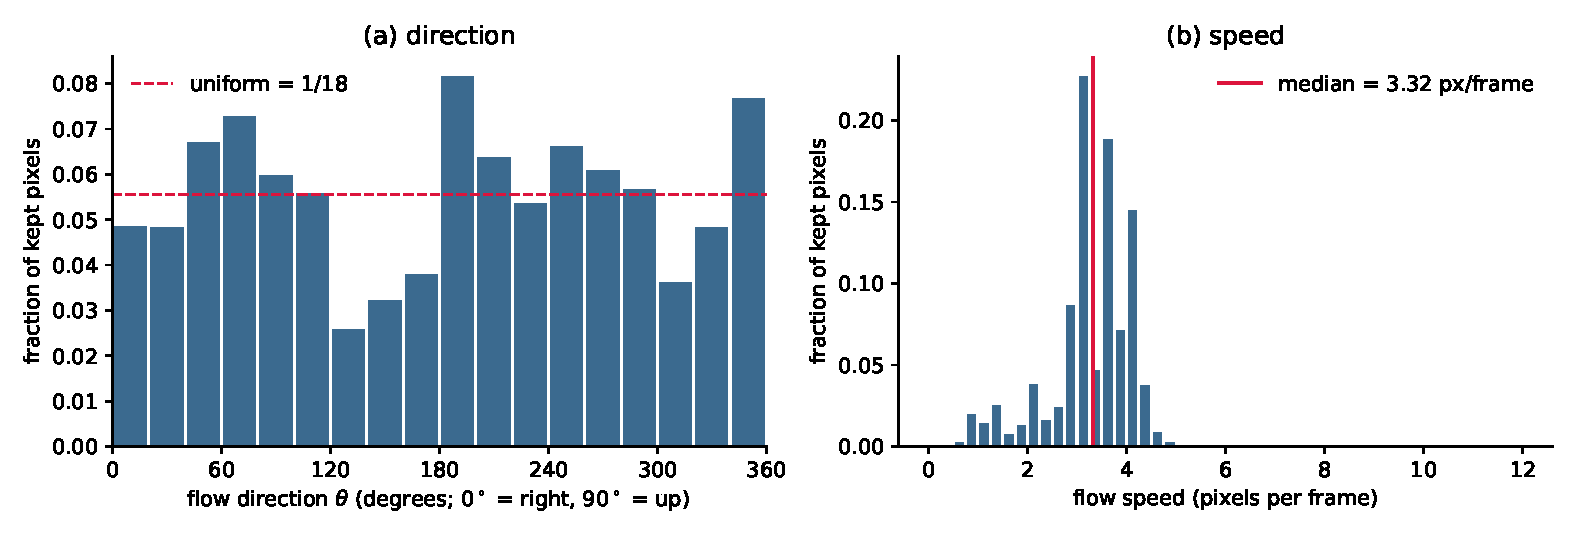
\includegraphics[width=0.97\linewidth]{fig1_flow.pdf}
\caption{Farneback optical flow on the first 50 training videos, pooled over $50\times19=950$ frame pairs; kept pixels (intensity $>0.2$ in both frames, flow magnitude $>0.5$ px): $N=103{,}050$. (a) direction $\theta=\operatorname{atan2}(-d_y,d_x)$, 18 bins of $20^\circ$ (fraction of kept pixels); the dashed line is the uniform level $1/18$. (b) speed in pixels per frame; \textbf{median speed $=3.32$ px/frame} (vertical line).}\label{fig:f1}
\end{figure}

\Q{Q2.1}{\textbf{Yes, mirrored and rotated trajectories are already familiar.} Figure~\ref{fig:f1}a is flat within sampling noise: the 18 bins lie between $0.026$ and $0.082$ around the uniform level $0.056$. This is what only 100 independent digit trajectories (50 videos $\times$ 2 digits) can produce: for 100 draws from a perfectly uniform direction law the largest relative deviation of an 18-bin histogram averages $0.88$ ($95^{\rm th}$ percentile $1.34$, Monte Carlo, 5000 draws), while we observe $0.53$. Mirroring sends $\theta\mapsto180^\circ-\theta$ and a $90^\circ$ rotation sends $\theta\mapsto\theta+90^\circ$ (4.5 bins). If every training video were mirrored, the histogram would be reflected about the vertical axis; if every video were rotated by $90^\circ$ it would be shifted by 4.5 bins; a flat histogram is unchanged by both, so the transformed directions are as common as the original ones. Quantitatively the total-variation distance between the histogram and its mirror image is $0.13$ (null mean $0.21$, $95^{\rm th}$ percentile $0.31$) and to its $90^\circ$-rotated copy $0.16$ (null $0.21$, $0.28$): no detectable asymmetry. Elastic bounces also reflect the velocity at the walls, so every trajectory visits mirror-image directions anyway. \emph{Speed:} the median is $3.32$ px/frame (inter-quartile range $3.00$--$3.89$, $5$--$95\%$: $1.41$--$4.32$; only $0.006\%$ of pixels exceed $8$ px/frame). The $2\times$ and $3\times$ videos therefore move about $6.6$ and $10.0$ px per frame \emph{between the frames the model sees} ($8.6$ and $13.0$ px for the $95^{\rm th}$-percentile speed): a range that never occurs at $1\times$. \emph{Overlap bias:} I recomputed Figure~\ref{fig:f1} after discarding every frame pair in which the two digits form one blob in either frame (443 of 950 pairs, where flow is unreliable): the median speed becomes $3.24$ px/frame, the largest relative deviation of the direction histogram from uniform $0.53$ (unchanged) and no pixel exceeds $8$ px/frame. The bias is too small to change the answer.}

\Q{Q2.2}{\begin{center}\small\begin{tabularx}{\linewidth}{@{}>{\raggedright\arraybackslash}p{2.2cm}>{\raggedright\arraybackslash}X>{\raggedright\arraybackslash}X@{}}\toprule
Transformation & Motion statistics & Digit appearance \\ \midrule
Mirror $M$ & unchanged: speeds identical, directions $\theta\to180^\circ-\theta$ (uniform $\Rightarrow$ same law) & \textbf{changed} (a mirrored 2 is not a 2) \\
Rotation $R$ & unchanged: speeds identical, $\theta\to\theta+90^\circ$ (same law) & \textbf{changed more} (stroke orientation too) \\
Speed-up $k\times$ & \textbf{changed}: displacement between seen frames $\times k$, directions unchanged & unchanged (same digits) \\ \bottomrule
\end{tabularx}\end{center}
Each transformation changes \emph{one} factor and leaves the other fixed: $M$ and $R$ change what the digits look like but keep the family of motions (a constant-velocity trajectory with elastic bounces in a square box is still valid after the symmetries of the square), while speed-up keeps the digits and changes the motion. A model that has learned \emph{how things move} should therefore be indifferent to $M$ and $R$ and should cope with $k\times$ as long as the motion is within its capacity; a failure under $M$/$R$ points to dependence on appearance, a failure under $k\times$ to unfamiliar motion or to architectural reach. That separation is what makes the three useful as a controlled experiment.}

% ------------------------------------------------------------------ 2. Baseline
\subsection*{2.\ Baseline: ConvLSTM}
Model A is implemented exactly as specified (pixel-unshuffle(4); two ConvLSTM layers, 64 hidden channels, $3\times3$ kernels, one convolution for all four gates, no peepholes; $1\times1$ conv $64\to16$, pixel-shuffle, sigmoid; 9-step free-running rollout, no teacher forcing, gradients through the fed-back predictions; states zero-initialised per video). It has \textbf{480,784} trainable parameters, as required. Training: Adam ($10^{-3}$), batch 32, 30 epochs, final-epoch weights, squared error averaged over pixels and available target frames then over videos.

\begin{table}[H]\centering\small
\caption{Test-set forecast error at $1\times$, $t=1$ (1000 test videos): per-horizon MSE, $E^{(5)}$ and trainable parameters.}\label{tab:t2}
\begin{tabular}{lrrrrrrr}\toprule
Predictor & MSE$_1$ & MSE$_2$ & MSE$_3$ & MSE$_4$ & MSE$_5$ & $E^{(5)}$ & Params \\ \midrule
Model A (mean of seeds 0, 1) & 0.0171 & 0.0203 & 0.0225 & 0.0241 & 0.0258 & 0.0220 & 480{,}784 \\
\quad seed 0 & 0.0173 & 0.0206 & 0.0228 & 0.0244 & 0.0260 & 0.0222 & 480{,}784 \\
\quad seed 1 & 0.0169 & 0.0201 & 0.0222 & 0.0239 & 0.0256 & 0.0217 & 480{,}784 \\
Blank & 0.0426 & 0.0426 & 0.0426 & 0.0425 & 0.0425 & 0.0426 & 0 \\
Copy-last & 0.0492 & 0.0604 & 0.0669 & 0.0708 & 0.0732 & 0.0641 & 0 \\
\bottomrule\end{tabular}
\end{table}
\begin{figure}[!htbp]\centering
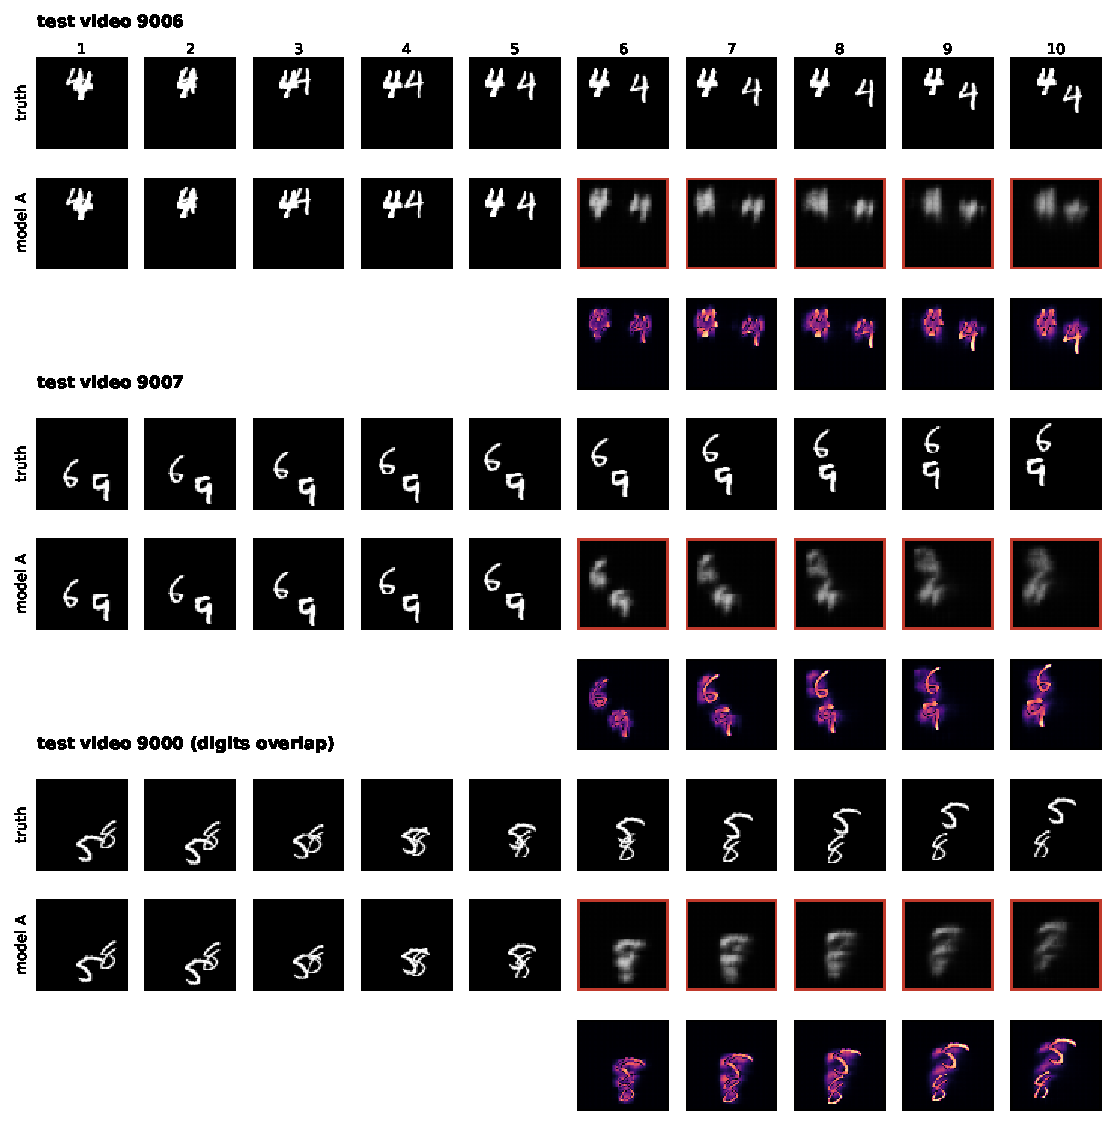
\includegraphics[width=0.86\linewidth]{fig2_predictions.pdf}
\caption{Model A (seed 0) on three test videos: 9006 and 9007 (digits never overlap in frames 6--10) and 9000 (digits overlap). For each: truth (frames 1--10), inputs 1--5 followed by the prediction of frames 6--10 (red frame), and the absolute error.}\label{fig:f2}
\end{figure}

\Q{Q2.3}{\textbf{Reach of model A $=8$ original pixels per time step.} Follow the longest path inside one step $\tau$ to the prediction $\hat x_{\tau+1}$. (i) One cell of the folded grid is 4 original pixels; a $3\times3$ convolution moves information by at most one cell, i.e.\ 4\,px. (ii) The new input $u_\tau$ is folded and enters layer~1, whose gates see a $3\times3$ neighbourhood of it ($1$ cell); layer~1's \emph{new} hidden state $h^{(1)}_\tau$ is the input of layer~2, whose $3\times3$ kernel adds one more cell ($1$ cell); the $1\times1$ output convolution, pixel-shuffle and sigmoid move nothing. Total $2$ cells $=8$\,px. (iii) The previous state $h^{(1)}_{\tau-1}$ takes the same route through layer~1's recurrent half and layer~2's input: $2$ cells; $h^{(2)}_{\tau-1}$ enters only layer~2's recurrent half: $1$ cell. The cell state $c$ is combined point-wise and moves nothing. The longest path is therefore $2\times4=\mathbf{8}$\,px, \emph{per step}; the recurrence lets state carry information further over several steps, but a digit that jumps farther than $8$\,px between two frames cannot be connected to its old position inside a single update. I checked this numerically: the gradient of one output pixel of one step with respect to $u_\tau$, $h^{(1)}_{\tau-1}$, $h^{(2)}_{\tau-1}$ is non-zero out to exactly $2$, $2$ and $1$ cells (\texttt{src/reach\_check.py}), i.e.\ $8$ px.}

\Q{Q2.4}{\textbf{Versus the references.} At $1\times$, model A (mean of seeds) has $E^{(5)}=0.0220$, against $0.0426$ for Blank ($-48\%$) and $0.0641$ for Copy-last ($-66\%$); it is better at every horizon ($\mathrm{MSE}_1$: $0.0171$ vs $0.0426$ and $0.0492$). \textbf{Error growth:} MSE rises steadily from $0.0171$ ($h{=}1$) to $0.0258$ ($h{=}5$), $+51\%$, i.e.\ about $0.0022$ per horizon, because every predicted frame is fed back and errors compound; Copy-last grows by a similar $+49\%$ ($0.0492\to0.0732$) and Blank stays flat. Even at $h{=}1$ model A is only $2.5\times$ better than Blank: Figure~\ref{fig:f2} shows that its forecasts are \emph{blurry}, at the right place but without sharp strokes, and they fade and spread with the horizon (the network hedges between possible shapes and positions). \textbf{Overlapping digits} (video 9000): the digits cross, and the forecast is a single smeared blob; the error map lights up along both digits' strokes, because the network cannot tell which stroke continues in which direction after the crossing and predicts an average of the possibilities. This is a failure of \emph{identity}, not a large increase of the average MSE: over the $586$ test videos whose digits overlap in frames 6--10, model A's $E^{(5)}$ is $0.0216$ against $0.0225$ for the other $414$ (seed-0/1 mean), since overlapping digits cover less area.}

\Q{Q2.5}{\textbf{Prediction, written before running any ``Testing the Baseline'' experiment} (verbatim from \texttt{predictions/Q2.5.md}, committed before \texttt{exp\_baseline.py} was run). \emph{Written before any Tables 3--4 or Figures 3--5 existed; I disclose that the training logs print the validation $E^{(2)}$ at $2\times$ and $3\times$, which I had seen (about 0.043 and 0.051 vs 0.022 for $E^{(5)}$ at $1\times$): the speed part is not fully blind, the mirror/rotation part is.}
\begin{quote}\small
\textbf{Mirror test.} Model A will mostly pass: the motion statistics are unchanged (only the digits' appearance changes), so I expect $E_M$ to be somewhat larger than $E^{(5)}$ (about 1.1--1.5$\times$) and $C_M$ clearly non-zero but small (roughly 10--30\,\% of $E^{(5)}$); both far better than Copy-last. It will not be exactly consistent.\\[2pt]
\textbf{Rotation test.} Model A will do worse than on the mirror test ($E_R$ about 1.5--3$\times$ $E^{(5)}$, $C_R$ larger than $C_M$): rotation changes the appearance more (stroke orientation changes; mirroring keeps vertical strokes vertical), and a ConvLSTM that partly memorised digit shapes to keep them sharp will blur or distort rotated digits. The motion rule itself should carry over, so I still expect it to stay better than Copy-last.\\[2pt]
\textbf{Speed.} It will be fine at $1\times$, degrade noticeably at $2\times$ (never seen in training and the fastest digits already reach the 8\,px limit; still better than Copy-last), and break down at $3\times$, where nearly every digit moves further than the 8\,px reach between seen frames: $E^{(2)}$ no better than Copy-last, and visible failures (a digit that stalls near its last seen position, ghosting/blur, or one that vanishes). So the breakdown speed should lie between $2\times$ and $3\times$, i.e.\ at an apparent displacement of about 8\,px per seen frame.
\end{quote}
\emph{After the fact (not part of the prediction):} mirror---right ($E_M/E^{(5)}=1.03$, $C_M=0.08\,E^{(5)}$; even better than guessed). Rotation---ordering right ($C_R>C_M$) but magnitude wrong ($E_R/E^{(5)}=1.08$, not $1.5$--$3$). Speed---failure type right (stall, blur), but the breakdown starts already at $2\times$ (worse than Blank) rather than between $2\times$ and $3\times$, and at $3\times$ model A is still better than Copy-last ($0.0703$ vs $0.0516$) although worse than Blank.}

% ------------------------------------------------------------------ 3. Testing the baseline
\subsection*{3.\ Testing the Baseline}
\begin{table}[H]\centering\small
\caption{Consistency gaps $C_T$ and transformed errors $E_T$ at $1\times$, $t=1$ on the 1000 test videos.}\label{tab:t3}
\begin{tabular}{lrrrrr}\toprule
Predictor & $E^{(5)}$ & $C_M$ & $E_M$ & $C_R$ & $E_R$ \\ \midrule
Model A (mean of seeds 0, 1) & 0.0220 & 0.00177 & 0.0226 & 0.00300 & 0.0237 \\
\quad seed 0 & 0.0222 & 0.00162 & 0.0228 & 0.00262 & 0.0237 \\
\quad seed 1 & 0.0217 & 0.00192 & 0.0224 & 0.00338 & 0.0237 \\
Blank & 0.0426 & 0 & 0.0426 & 0 & 0.0426 \\
Copy-last & 0.0641 & 0 & 0.0641 & 0 & 0.0641 \\
\bottomrule\end{tabular}
\end{table}
\begin{figure}[!htbp]\centering
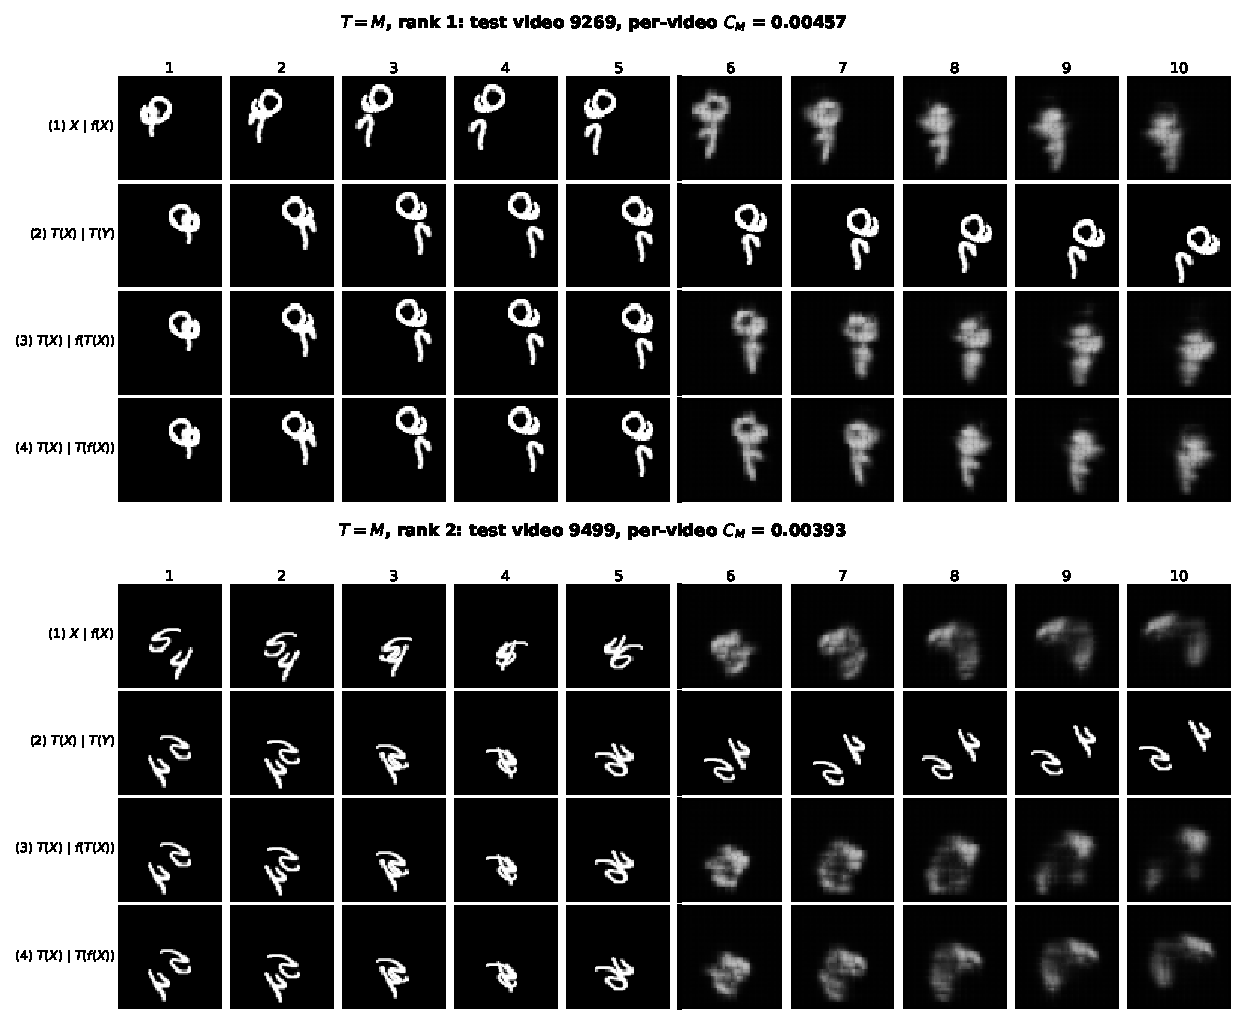
\includegraphics[width=0.8\linewidth]{fig3_M.pdf}\\[2pt]
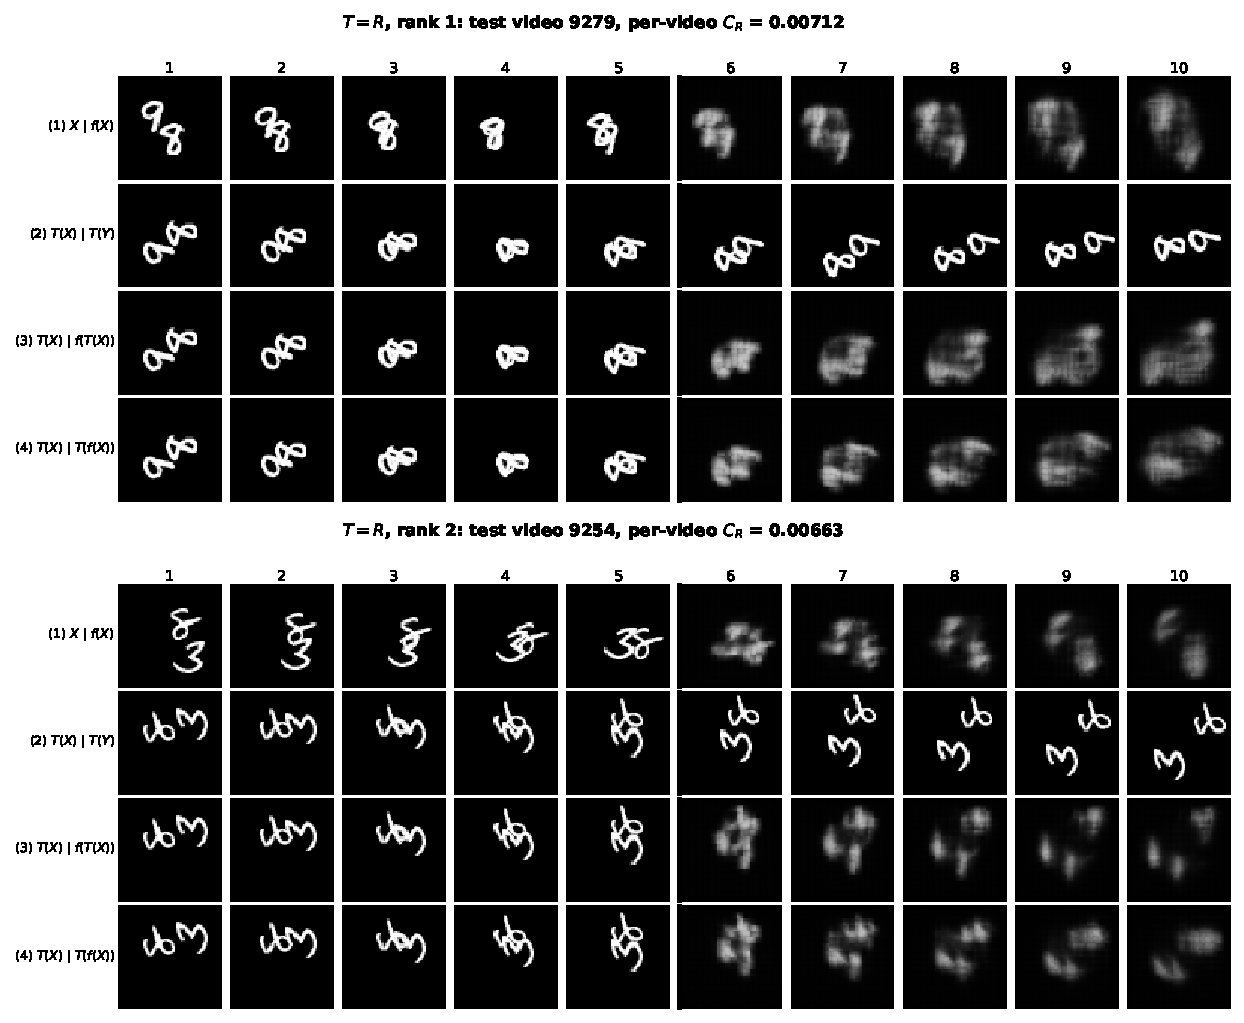
\includegraphics[width=0.8\linewidth]{fig3_R.pdf}
\caption{Model A (seed 0), $1\times$, $t=1$. Top: $T=M$, the two test videos with the largest per-video $C_M$ (9269, 9499); bottom: $T=R$, largest per-video $C_R$ (9279, 9254). Columns 1--5 are inputs, 6--10 the five future frames; rows (1) $X\,|\,f(X)$, (2) $T(X)\,|\,T(Y)$, (3) $T(X)\,|\,f(T(X))$, (4) $T(X)\,|\,T(f(X))$. Animated GIFs stepping through the five horizons with the same four rows (last input $|$ horizon $h$): \texttt{figures/gifs/fig3\_M\_rank1\_video9269.gif}, \texttt{fig3\_M\_rank2\_video9499.gif}, \texttt{fig3\_R\_rank1\_video9279.gif}, \texttt{fig3\_R\_rank2\_video9254.gif}.}\label{fig:f3}
\end{figure}
\begin{figure}[!htbp]\centering
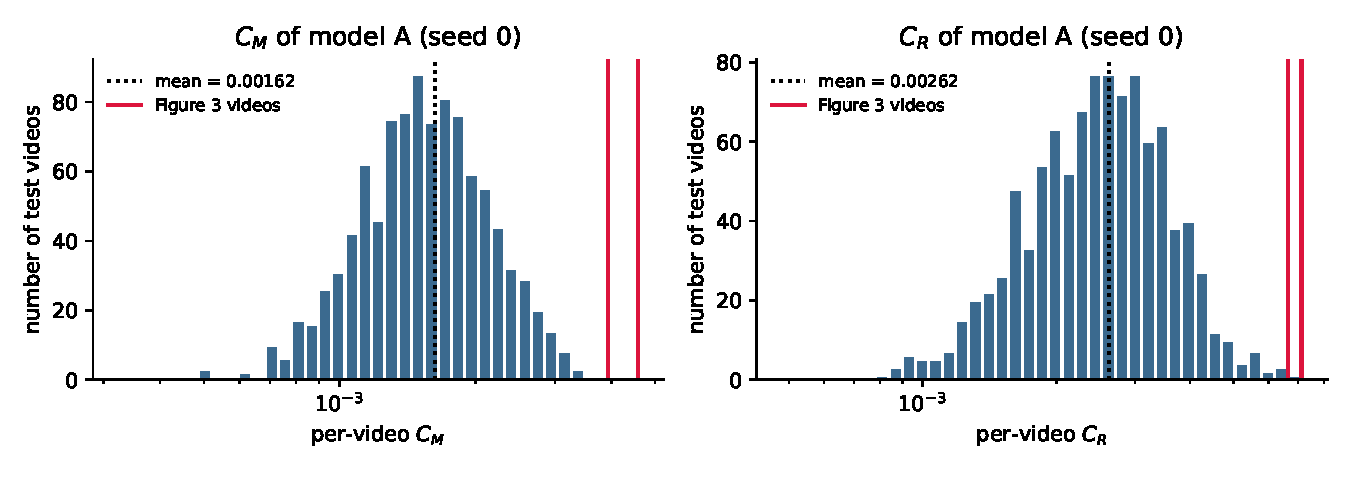
\includegraphics[width=0.85\linewidth]{fig4_hist.pdf}
\caption{Per-video $C_M$ (left) and $C_R$ (right) of model A (seed 0) over the 1000 test videos (log-scaled axis); red lines: the videos shown in Figure~\ref{fig:f3}; dotted: mean.}\label{fig:f4}
\end{figure}

\Q{Q2.6}{\textbf{Blank} (all zeros) and \textbf{Copy-last} are exactly consistent ($C_M=C_R=0$ in Table~\ref{tab:t3}) because both commute with every pixel permutation: $T(0)=0$, and copying the last frame commutes with mirroring or rotating it. So $C_T$ measures only whether the predictor treats a scene and its transformed copy \emph{alike}, never whether the prediction is \emph{right}: Blank is perfectly consistent and has $E^{(5)}=0.0426$, almost twice model A's. Consistency is necessary for a symmetric rule but not sufficient, and a blurrier forecast is more consistent almost by construction, so a small $C_T$ can come from vagueness. $E_T$, which compares the prediction for the transformed scene with the transformed truth, must always be read next to it. For model A: $C_M=0.00177$, $E_M=0.0226$ ($1.03\times E^{(5)}$), $C_R=0.00300$, $E_R=0.0237$ ($1.08\times$) --- consistent \emph{and} accurate, both far better than Copy-last ($0.0641$).}

\Q{Q2.7}{\textbf{Video 9279, $T=R$} (bottom of Figure~\ref{fig:f3}, rows 3 vs 4; seed-0 model A, $1\times$). Two digits (9 and 8) overlap in the last input frames and then separate. The truth (row 2) has its ink centroid moving $1.46$ px/frame. Row 4, $T(f(X))$ (original orientation), tracks it: centroid speed $1.44$ px/frame, the pair separates and drifts. Row 3, $f(T(X))$ (rotated input), \emph{stalls}: the centroid moves only $0.27$ px/frame (a fifth), ending $\approx5$\,px from where row 4 puts it, and the forecast becomes a horizontally smeared single blob whose total ink grows from $310$ ($h{=}1$) to $421$ ($h{=}5$) while the truth stays at $255$--$273$, and whose spread grows from $12.7$ to $18.0$ px (truth: $9.3\to12.4$). So the model's account changes from ``two digits that separate and move on'' to ``one digit-sized blob that stays put and blurs''. The other three videos disagree less: for $T=M$, video 9269, the two rows have the same centroid speed ($2.44$ vs $2.42$ px/frame against the true $3.29$) and differ mainly in blur details (centroid gap $1.5$ px).}

\Q{Q2.8}{\textbf{Yes, for model A rotation is harder than mirroring, and the difference comes from appearance, not motion.} Table~\ref{tab:t3}: $C_R=0.00300$ vs $C_M=0.00177$ ($1.7\times$) and $E_R-E^{(5)}=0.00174$ vs $E_M-E^{(5)}=0.00064$ ($2.7\times$). By Q2.1 neither transformation changes the motion statistics: directions are uniform and the speed is unchanged, so a purely motion-based rule would treat both alike. By Q2.2 both change the appearance, rotation more: $M$ flips the digits but keeps vertical strokes vertical and the stroke-orientation statistics roughly the same, whereas $R$ interchanges horizontal and vertical strokes, so rotated digits are further from anything seen in training. The part of the forecast that is carried by digit shape (keeping strokes sharp, resolving overlaps) is the part that degrades, as the stalled, blurred blob in Q2.7 shows. Model B (trained with $G$) tests this directly: if appearance is the cause, symmetry augmentation should shrink the gap (Table~\ref{tab:t5}). The gap itself is small compared with the speed failure below, so model A's motion rule is largely orientation-agnostic.}

\begin{table}[H]\centering\small
\caption{Speed test on the 1000 test videos ($t=1$). $E^{(2)}$ uses only the first two horizons (the only ones that exist at $3\times$).}\label{tab:t4}
\begin{tabular}{lrrrrr}\toprule
Predictor & $E^{(2)}$ 1$\times$ & $E^{(2)}$ 2$\times$ & $E^{(2)}$ 3$\times$ & $E^{(5)}$ 1$\times$ & $E^{(5)}$ 2$\times$ \\ \midrule
Model A (mean of seeds 0, 1) & 0.0187 & 0.0444 & 0.0516 & 0.0220 & 0.0492 \\
\quad seed 0 & 0.0189 & 0.0433 & 0.0508 & 0.0222 & 0.0477 \\
\quad seed 1 & 0.0185 & 0.0455 & 0.0524 & 0.0217 & 0.0507 \\
Copy-last & 0.0548 & 0.0661 & 0.0703 & 0.0641 & 0.0719 \\
Blank & 0.0426 & 0.0425 & 0.0426 & 0.0426 & 0.0425 \\
\bottomrule\end{tabular}
\end{table}
\begin{figure}[!htbp]\centering
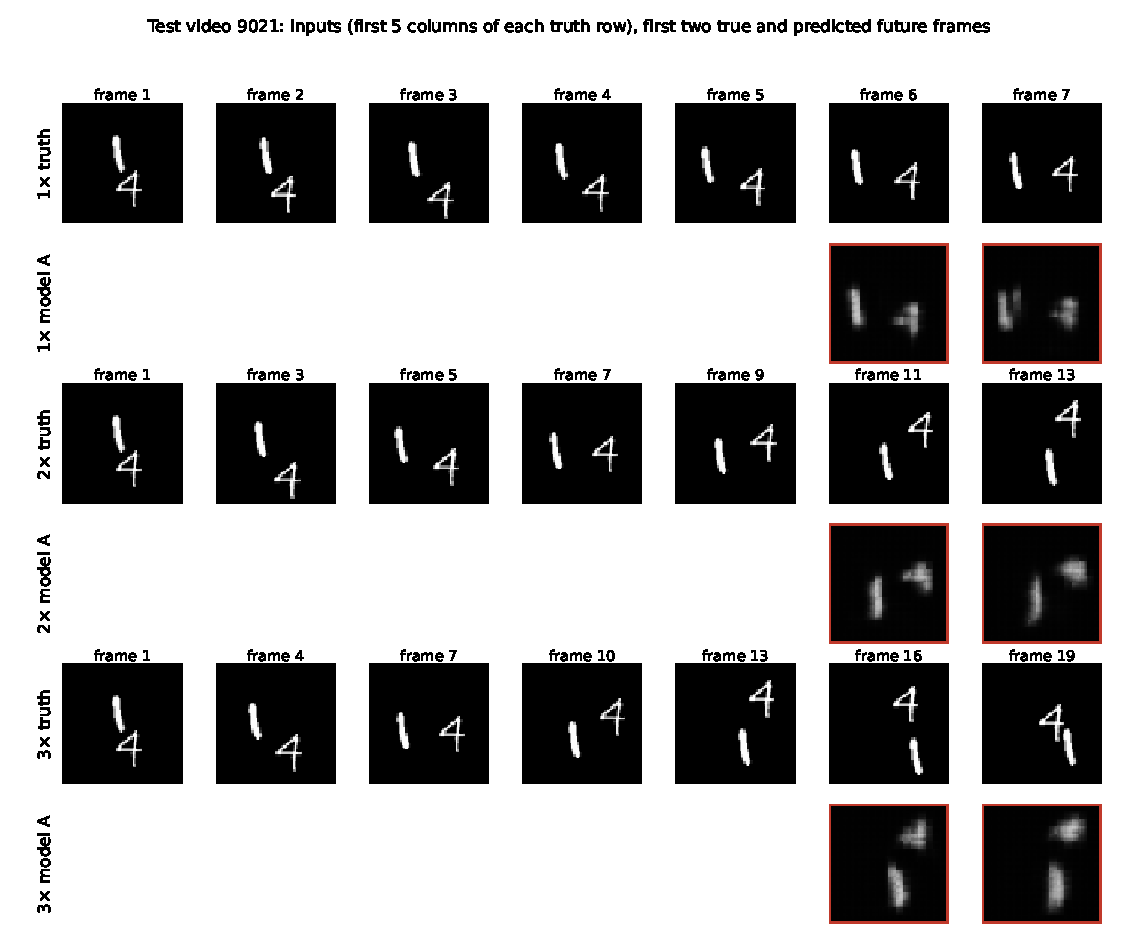
\includegraphics[width=0.93\linewidth]{fig5_speed.pdf}
\caption{Model A (seed 0), test video 9021 (digits do not overlap in any displayed true frame): five input frames, first two true future frames, and the first two predicted frames (red) at $1\times$, $2\times$, $3\times$ ($t=1$; frame numbers above each column).}\label{fig:f5}
\end{figure}

\Q{Q2.9}{\textbf{Where it falls apart.} $1\times$ is fine; at $2\times$ the error already jumps to $E^{(2)}=0.0444$ ($2.4\times$ its $1\times$ value $0.0187$; better than Copy-last $0.0661$ but \emph{worse} than Blank $0.0426$) and at $3\times$ it is $0.0516$ (Copy-last $0.0703$, Blank $0.0426$); the $E^{(5)}$ at $2\times$ is $0.0492$ against $0.0220$ at $1\times$. Table~S1 (row A, in Section 5) measures what goes wrong: from the last input frame to the first forecast, a digit's centroid truly moves $3.6$, $7.1$, $10.4$ px at $1\times$, $2\times$, $3\times$; model A moves its predicted digit by $3.3$--$3.4$ ($95\%$ of the truth), $2.5$ ($39\%$) and $1.8$--$2.3$ px ($19$--$25\%$). So \emph{it does not agree with my reach estimate}: with $8$\,px reach, $2\times$ (true displacement $7.1$\,px for the median digit, $<8$) should still work for most digits, yet the failure already starts there, and by $3\times$ ($10.4>8$) it is nearly total. What the estimate missed: the reach is a \emph{maximum} possible path, not what the network has learned to use. Trained only on displacements of about $3$--$4$\,px, the outer cells of its kernels (those that would carry a $7$\,px jump) have never been needed, so the effective reach is smaller than the nominal one, and $2\times$ is also simply unfamiliar. \textbf{What the failure looks like (Figure~\ref{fig:f5}):} \emph{stalling} and \emph{blur}: at $2\times$ and $3\times$ the digits appear washed out and close to the position where they were last seen, with a faint trailing smear toward the true position, but they do not move $k\times$ as far. I see no duplicated digit and no complete vanishing (intensity is lower but present). A stalled digit means the network failed to link the old position held in its state with the new position (it falls back on ``no motion''); a blur means it spreads probability over positions it cannot distinguish, as expected under squared error.}

\Q{Q2.10}{\textbf{No, not from these results alone.} Model A has a single training speed \emph{and} a single, small reach, so the two explanations predict the same thing, a failure at $2\times$ and $3\times$: ``fast motion never appeared in training'' and ``it is beyond the model's reach'' are confounded. The displacement numbers only hint: $2\times$ ($7.1$ px, below the nominal reach) fails, favouring unfamiliarity at least there, but the effective reach is unknown. \textbf{An experiment that separates them:} train the same architecture on all three speeds (model C: familiarity restored, reach unchanged) and a larger-reach architecture (model D) on the same data, and evaluate each at $2\times$ and $3\times$: if C fixes a speed, that failure was unfamiliar motion; if C still fails where D succeeds, it was reach. A cleaner variant is the \emph{reach-only} control, a larger-reach model trained at $1\times$ only: if it still fails at $2\times$, unfamiliarity is the cause, even though the displacement is now within reach.}

% ============================================================== QUESTION 2 (part b)
% ------------------------------------------------------------------ 4. What can data fix?
\subsection*{4.\ What Can Data Fix?}
Models B and C each change one thing relative to A; model D changes only the architecture relative to C; D+B (optional) adds symmetry augmentation to D. All were trained with the protocol of \emph{Training and evaluation} (seeds 0 and 1). Symmetry augmentation draws $g\in G$ uniformly per training window (including the identity) and applies it to input and target; speed augmentation draws $k\in\{1,2,3\}$ and then $t$ uniformly from the allowed starts ($14/8/2$).

\Q{Q2.11}{\textbf{Prediction, written before training B, C or D} (verbatim from \texttt{predictions/Q2.11.md}, committed before training B, C or D; no candidate design of D had been trained either).
\begin{quote}\small
Testing the Baseline showed that model A is almost consistent under mirror and rotation ($E_M$ and $E_R$ within about 8\,\% of $E^{(5)}$, $C_M$ and $C_R$ about 8\,\% and 14\,\% of $E^{(5)}$), but that at $2\times$ and $3\times$ its $E^{(2)}$ (0.044, 0.052) is more than twice its $1\times$ value and worse than the all-zero Blank predictor; its reach (8\,px) is below the apparent displacement at $3\times$ (about 10\,px) and borderline at $2\times$ (about 6.6\,px typical, 8+\,px for the fastest digits).\\[2pt]
\textbf{Prediction (three sentences).} Model B (symmetry augmentation) will lower $C_M$, $C_R$, $E_M$ and $E_R$ only slightly, because there is little appearance gap left to close, and will not help at $2\times$ or $3\times$. Model C (speed augmentation, same reach) will fix most of the $2\times$ failure (unfamiliar motion) but will still fail clearly at $3\times$, where the apparent displacement exceeds its 8\,px reach. Model D (reach 16\,px, with speed augmentation) will fix $3\times$ as well, at little or no cost in $1\times$ accuracy.
\end{quote}
\emph{After the fact:} B---right. C---right at $2\times$, \textbf{wrong at $3\times$}: C also fixes most of the $3\times$ failure ($E^{(2)}$ $0.0516\to0.0332$). D---it fixes $3\times$, but only slightly better than C ($0.0320$), and not ``at little cost'' at $1\times$: the cost ($E^{(5)}$ $0.0220\to0.0267$) is already paid by C. The reach I estimated was \emph{not} the main bottleneck (see Q2.13).}

\begin{table}[H]\centering\scriptsize\setlength{\tabcolsep}{2.5pt}
\caption{Models A--D (and optional D+B) on the 1000 test videos, both seeds. $E^{(5)}$, $C_T$, $E_T$ at $1\times$, $t=1$; $E^{(2)}$ at $1\times$, $2\times$, $3\times$. Times: see hardware in the text.}\label{tab:t5}
\begin{tabular}{lrrrrrrrrrrr}\toprule
Model & $E^{(5)}$ & $C_M$ & $E_M$ & $C_R$ & $E_R$ & $E^{(2)}_{1\times}$ & $E^{(2)}_{2\times}$ & $E^{(2)}_{3\times}$ & Params & s/epoch & Infer. (s) \\ \midrule
A baseline (mean) & 0.0220 & 0.00177 & 0.0226 & 0.00300 & 0.0237 & 0.0187 & 0.0444 & 0.0516 & 480{,}784 & 13.6 & 0.586 \\
\quad seed 0 & 0.0222 & 0.00162 & 0.0228 & 0.00262 & 0.0237 & 0.0189 & 0.0433 & 0.0508 & 480{,}784 & 13.6 & 0.596 \\
\quad seed 1 & 0.0217 & 0.00192 & 0.0224 & 0.00338 & 0.0237 & 0.0185 & 0.0455 & 0.0524 & 480{,}784 & 13.5 & 0.576 \\
\midrule
B +sym.\ aug. (mean) & 0.0223 & 0.00128 & 0.0223 & 0.00153 & 0.0223 & 0.0187 & 0.0447 & 0.0509 & 480{,}784 & 23.1 & 0.573 \\
\quad seed 0 & 0.0230 & 0.00128 & 0.0231 & 0.00163 & 0.0229 & 0.0192 & 0.0450 & 0.0520 & 480{,}784 & 23.1 & 0.575 \\
\quad seed 1 & 0.0216 & 0.00128 & 0.0216 & 0.00144 & 0.0216 & 0.0182 & 0.0444 & 0.0498 & 480{,}784 & 23.1 & 0.572 \\
\midrule
C +speed aug. (mean) & 0.0269 & 0.00109 & 0.0271 & 0.00206 & 0.0279 & 0.0234 & 0.0289 & 0.0332 & 480{,}784 & 14.0 & 0.574 \\
\quad seed 0 & 0.0274 & 8.76e-04 & 0.0277 & 0.00166 & 0.0283 & 0.0240 & 0.0295 & 0.0335 & 480{,}784 & 14.0 & 0.568 \\
\quad seed 1 & 0.0263 & 0.00130 & 0.0265 & 0.00245 & 0.0274 & 0.0228 & 0.0283 & 0.0330 & 480{,}784 & 14.0 & 0.579 \\
\midrule
D larger reach (mean) & 0.0267 & 0.00109 & 0.0269 & 0.00235 & 0.0278 & 0.0238 & 0.0282 & 0.0320 & 603{,}088 & 20.8 & 0.648 \\
\quad seed 0 & 0.0267 & 0.00129 & 0.0269 & 0.00272 & 0.0279 & 0.0238 & 0.0282 & 0.0320 & 603{,}088 & 18.8 & 0.650 \\
\quad seed 1 & 0.0267 & 8.93e-04 & 0.0269 & 0.00199 & 0.0278 & 0.0239 & 0.0283 & 0.0319 & 603{,}088 & 22.8 & 0.646 \\
\midrule
D+B (mean) & 0.0276 & 4.55e-04 & 0.0277 & 4.78e-04 & 0.0277 & 0.0247 & 0.0295 & 0.0330 & 603{,}088 & 33.0 & 0.657 \\
\quad seed 0 & 0.0275 & 5.96e-04 & 0.0275 & 5.68e-04 & 0.0276 & 0.0246 & 0.0295 & 0.0328 & 603{,}088 & 35.7 & 0.651 \\
\quad seed 1 & 0.0278 & 3.15e-04 & 0.0278 & 3.88e-04 & 0.0278 & 0.0249 & 0.0296 & 0.0332 & 603{,}088 & 30.2 & 0.663 \\
\midrule
Copy-last & 0.0641 & 0 & 0.0641 & 0 & 0.0641 & 0.0548 & 0.0661 & 0.0703 & 0 & -- & 1.07e-04 \\
\bottomrule\end{tabular}
\end{table}
{\footnotesize\emph{Timing note.} Times are the logged means over the 30 epochs and the timed inference of the final weights. Some logged epochs of D (seed 0) and D+B (seed 1) were up to $2\times$ faster than the rest (GPU/WSL power-state or clock changes during that period), so I also re-timed all five architectures in a controlled run (idle GPU, seed 0, mean of epochs 2--4): A $10.9$\,s, B $17.1$\,s, C $10.7$\,s, D $14.5$\,s, D+B $20.5$\,s per epoch; the ordering (augmentation overhead of the per-sample symmetry loop; D's dilated, wider layers) is the same as in the table. The inference times of A, B, C are equal ($\approx0.58$\,s for 1000 videos) because they share the architecture; D's is $\approx0.65$\,s.}\par\medskip

\Q{Q2.12}{\textbf{Model D} is the same 9-step free-running ConvLSTM as A (patch 4, two layers, input/output shapes, no teacher forcing, same training protocol), with a different spatial configuration: hidden width $72$ (instead of 64) and a \emph{dilated} second layer: layer~1 is a $3\times3$ convolution (dilation 1), layer~2 a $3\times3$ convolution with \textbf{dilation 2} (zero padding 2 keeps the $16\times16$ size). It has $603{,}088$ trainable parameters ($1.25\times$ A; limit $721{,}176$). The design was chosen on the \emph{validation split only} from six candidates (dilated, 5$\times$5-kernel, wider and patch-8 variants; all within the parameter limit and with reach $>8$\,px), each trained for 12 epochs with the C protocol (seed 0) and ranked by the pre-declared score mean($E^{(5)}$@$1\times$, $E^{(2)}$@$2\times$, $E^{(2)}$@$3\times$) (\texttt{results/d\_design.json}); this one scored best ($0.0316$ vs.\ $0.0339$ for the runner-up). Caveat: three candidates (d2, d4, d5 in \texttt{results/d\_design.json}) were still on the initial loss plateau after 12 epochs, so the choice partly reflects how quickly a design starts learning.\\[2pt]
\textbf{Reach, same method as Q2.3.} Radius of a dilated $3\times3$ convolution $=d\cdot(k-1)/2$ cells: layer~1 $1$ cell, layer~2 $2$ cells. Longest paths in one step: new input $u_\tau\to$ layer~1 ($1$) $\to$ layer~2 ($2$) $=3$ cells; $h^{(1)}_{\tau-1}\to$ layer~1 ($1$) $\to$ layer~2 ($2$) $=3$ cells; $h^{(2)}_{\tau-1}\to$ layer~2 recurrent ($2$) $=2$ cells; the $1\times1$ convolution, pixel-shuffle and sigmoid add nothing. With one cell $=4$ px the reach is $3\times4=\mathbf{12}$\,px, strictly larger than A's $8$\,px (the offsets $\{-1,0,1\}+\{-2,0,2\}$ cover $-3..3$ without gaps, so no ``checkerboard'' blind spots). Verified numerically with autograd (\texttt{src/reach\_check.py}: $3,3,2$ cells $\Rightarrow$ $12$\,px). Compared with the displacements of Q2.9: $12>10.4$\,px, so D can reach the median digit even at $3\times$ (A could not).}

\Q{Q2.13}{\textbf{Labels (Table~\ref{tab:t5}, Table~S1; means of seeds).}
\begin{itemize}[leftmargin=*,itemsep=1pt,topsep=2pt]
\item \emph{Appearance} (mirror/rotation, $1\times$): small in A and removed by B. $E_R-E^{(5)}$: A $0.0017$ (A: $E_R=0.0237$) $\to$ B $-0.0001$ ($E_R=0.0223$); $C_R$: $0.00300\to0.00153$; $C_M$: $0.00177\to0.00128$. Models without symmetry augmentation (C, D) keep a gap ($E_R-E^{(5)}=0.0010$--$0.0012$), B closes it, which is why I attribute it to appearance.
\item \emph{Unfamiliar motion} ($2\times$ and $3\times$): B does not help ($E^{(2)}$ $0.0447$, $0.0509$ vs A's $0.0444$, $0.0516$) but C does: $E^{(2)}_{2\times}$ $0.0444\to0.0289$ ($-35\%$), $E^{(2)}_{3\times}$ $0.0516\to0.0332$ ($-36\%$), and the digits' displacement at $2\times$ rises from $39\%$ (A) to $84\%$ of the truth (Table~S1), at $3\times$ from $22\%$ to $72\%$. Same architecture, same reach, only the training speeds changed: this is the dominant cause, at both speeds.
\item \emph{Architectural reach}: D versus C changes only the architecture: $E^{(2)}_{3\times}$ $0.0332\to0.0320$ ($-3.7\%$, lower in both seeds: C $0.0335, 0.0330$; D $0.0320, 0.0319$), $E^{(2)}_{2\times}$ $0.0289\to0.0282$ ($-2.4\%$); displacement at $3\times$ $72\%\to77\%$. A real but small contribution, mainly at $3\times$, where the true displacement ($10.4$\,px) exceeds A's reach.
\end{itemize}
\textbf{If C still did badly at $3\times$ while D did well} that would show that the failure was \emph{architectural}: more training data cannot carry information further than the architecture allows, because the output at a pixel is a function of a bounded set of input cells (the gradient with respect to anything beyond the reach is exactly zero, as checked numerically) and training can only change how the available paths are weighted, never create new ones. Here it did not happen: C already reaches $72\%$ of the true $3\times$ displacement with its nominal 8\,px reach, so, as Q2.9 anticipated, the nominal reach overstates the true limitation once the network has seen fast motion. That \emph{I predicted otherwise in Q2.11 was wrong}.}

\Q{Q2.14}{\textbf{Yes, there is a cost at $1\times$, and it comes from speed augmentation, not from the architecture.} $E^{(5)}$ at $1\times$: A $0.0220$, B $0.0223$ ($+1.7\%$, within the seed spread $0.0216$--$0.0230$), C $0.0269$ ($+22\%$), D $0.0267$ ($+22\%$); $E^{(2)}$ at $1\times$: A $0.0187$, C $0.0234$ ($+25\%$), D $0.0238$ ($+27\%$). The network now spends its fixed capacity and 30 epochs on three speeds, so it is less sharp at the one it was good at. \textbf{Worth it?} For a forecaster that must work at several speeds, yes: $-36\%/-38\%$ error at $2\times/3\times$ (D) for $+22\%$ at $1\times$; A at $2\times$ and $3\times$ is worse than predicting a blank frame ($0.0426$), whereas C and D beat Blank by about $32\%$ at $2\times$ and $22$--$25\%$ at $3\times$. For a $1\times$-only use case it is not worth it. B is essentially free in accuracy and improves consistency (Q2.15), so yes for B. D costs $\approx1.1\times$ inference time over C and $\approx1.4\times$ epoch time, for $-3$ to $-4\%$ error at $3\times$ and no gain at $1\times$.}

% ------------------------------------------------------------------ 5. Final model
\subsection*{5.\ The Final Model}
\textbf{Why $\bar f$ has $C_M=C_R=0$ exactly.} Let $T\in\{M,R\}\subset G$ and $f$ any forecaster. $G$ is a group, so for fixed $T$ the map $g\mapsto h=gT$ is a bijection of $G$, and $g^{-1}=Th^{-1}$. Then
\[
\bar f(T(X))=\tfrac18\sum_{g}g^{-1}\big(f(gT(X))\big)=\tfrac18\sum_{h}T\,h^{-1}\big(f(h(X))\big)=T\Big(\tfrac18\sum_{h}h^{-1}(f(h(X)))\Big)=T(\bar f(X)),
\]
because $T$ only permutes pixels (a linear map that commutes with the average). Hence $C_T=\mathrm{MSE}(\bar f(T(X)),T(\bar f(X)))=0$ for every $f$, and also $E_T=\mathrm{MSE}(T\bar f(X),T(Y))=E^{(5)}$. In floating point, the inputs $gT(X)$ and $h(X)$ are bitwise identical (pure data movement), so every call of $f$ gives identical outputs, and only the order of the eight summands differs; I accumulate in float64, so the measured $C_M$, $C_R$ are $0$ (to the printed precision: exactly $0.00$).

\textbf{Choice of the final model.} The final model is \textbf{D wrapped as a symmetrised forecaster}. I also trained D+B (optional) and chose between them on the \emph{validation} split with the wrapped forecasters: $E^{(5)}$ $0.0264$ (sym.\ D) vs $0.0272$ (sym.\ D+B) (mean of seeds): D is better, and it is also cheaper to train, so the final model is sym.\ D.

\begin{table}[H]\centering\scriptsize\setlength{\tabcolsep}{2.5pt}
\caption{Symmetrised forecasters $\bar f$ (eq.~7) on the test set. Training time is that of the underlying learned model; inference includes all 8 transformations, forward passes, inverse transformations and averaging.}\label{tab:t6}
\begin{tabular}{lrrrrrrrrrrr}\toprule
Model & $E^{(5)}$ & $C_M$ & $E_M$ & $C_R$ & $E_R$ & $E^{(2)}_{1\times}$ & $E^{(2)}_{2\times}$ & $E^{(2)}_{3\times}$ & Params & s/epoch & Infer. (s) \\ \midrule
sym.\ B (mean) & 0.0217 & 0.00e+00 & 0.0217 & 0.00e+00 & 0.0217 & 0.0183 & 0.0440 & 0.0500 & 480{,}784 & 23.1 & 2.60 \\
\quad seed 0 & 0.0223 & 0.00e+00 & 0.0223 & 0.00e+00 & 0.0223 & 0.0187 & 0.0443 & 0.0511 & 480{,}784 & 23.1 & 2.77 \\
\quad seed 1 & 0.0210 & 0.00e+00 & 0.0210 & 0.00e+00 & 0.0210 & 0.0178 & 0.0437 & 0.0488 & 480{,}784 & 23.1 & 2.44 \\
\midrule
sym.\ D (mean) & 0.0265 & 0.00e+00 & 0.0265 & 0.00e+00 & 0.0265 & 0.0237 & 0.0282 & 0.0318 & 603{,}088 & 20.8 & 3.13 \\
\quad seed 0 & 0.0264 & 0.00e+00 & 0.0264 & 0.00e+00 & 0.0264 & 0.0236 & 0.0281 & 0.0319 & 603{,}088 & 18.8 & 3.08 \\
\quad seed 1 & 0.0267 & 0.00e+00 & 0.0267 & 0.00e+00 & 0.0267 & 0.0239 & 0.0282 & 0.0318 & 603{,}088 & 22.8 & 3.19 \\
\midrule
sym.\ D+B (mean) & 0.0275 & 0.00e+00 & 0.0275 & 0.00e+00 & 0.0275 & 0.0246 & 0.0294 & 0.0329 & 603{,}088 & 33.0 & 3.14 \\
\quad seed 0 & 0.0273 & 0.00e+00 & 0.0273 & 0.00e+00 & 0.0273 & 0.0244 & 0.0294 & 0.0327 & 603{,}088 & 35.7 & 3.09 \\
\quad seed 1 & 0.0276 & 0.00e+00 & 0.0276 & 0.00e+00 & 0.0276 & 0.0248 & 0.0294 & 0.0331 & 603{,}088 & 30.2 & 3.20 \\
\bottomrule\end{tabular}
\end{table}
\begin{figure}[!htbp]\centering
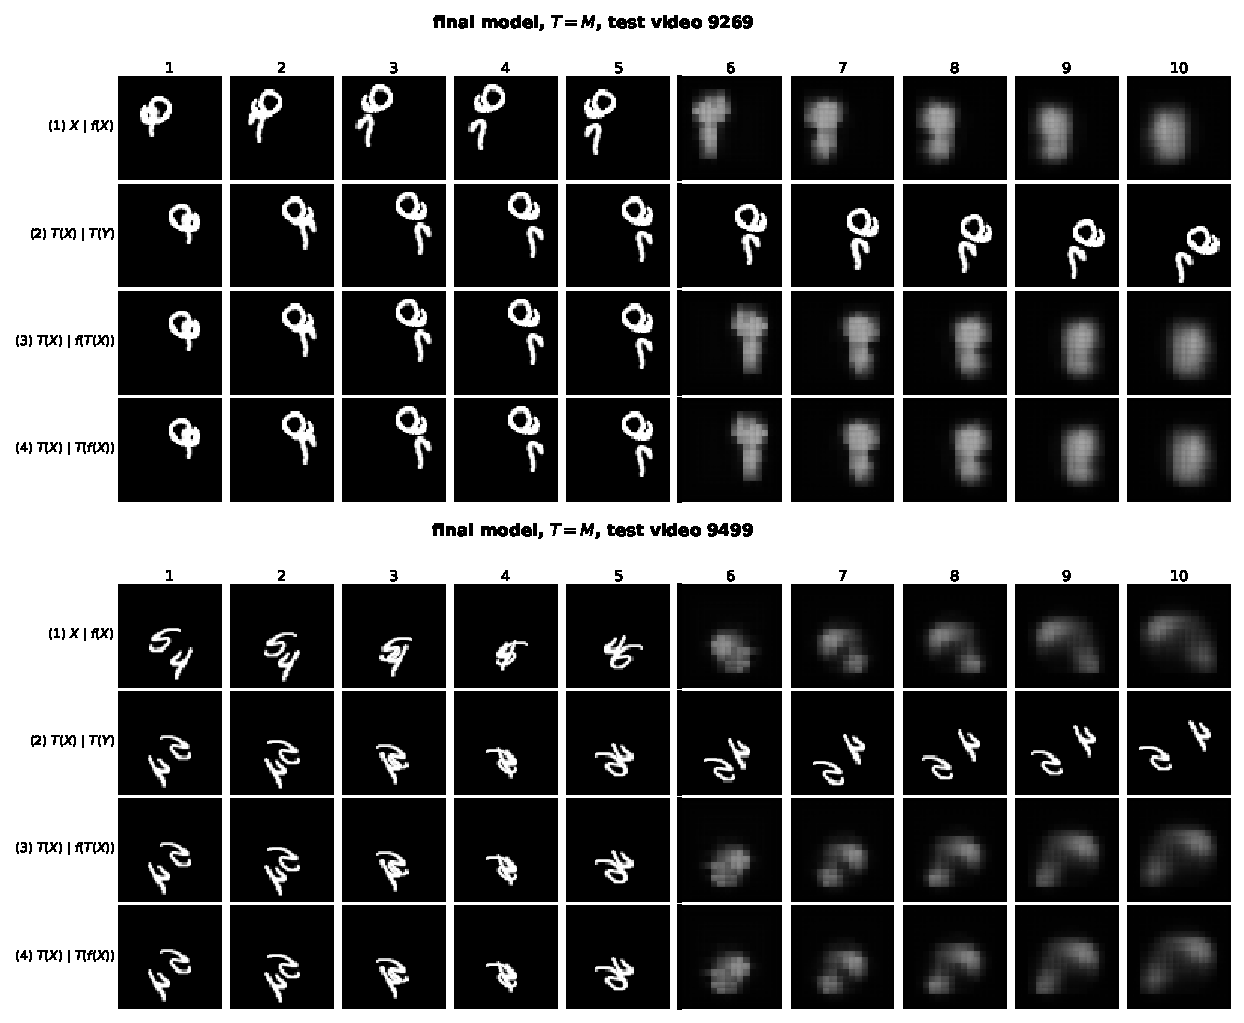
\includegraphics[width=0.88\linewidth]{fig6a_M.pdf}\\[2pt]
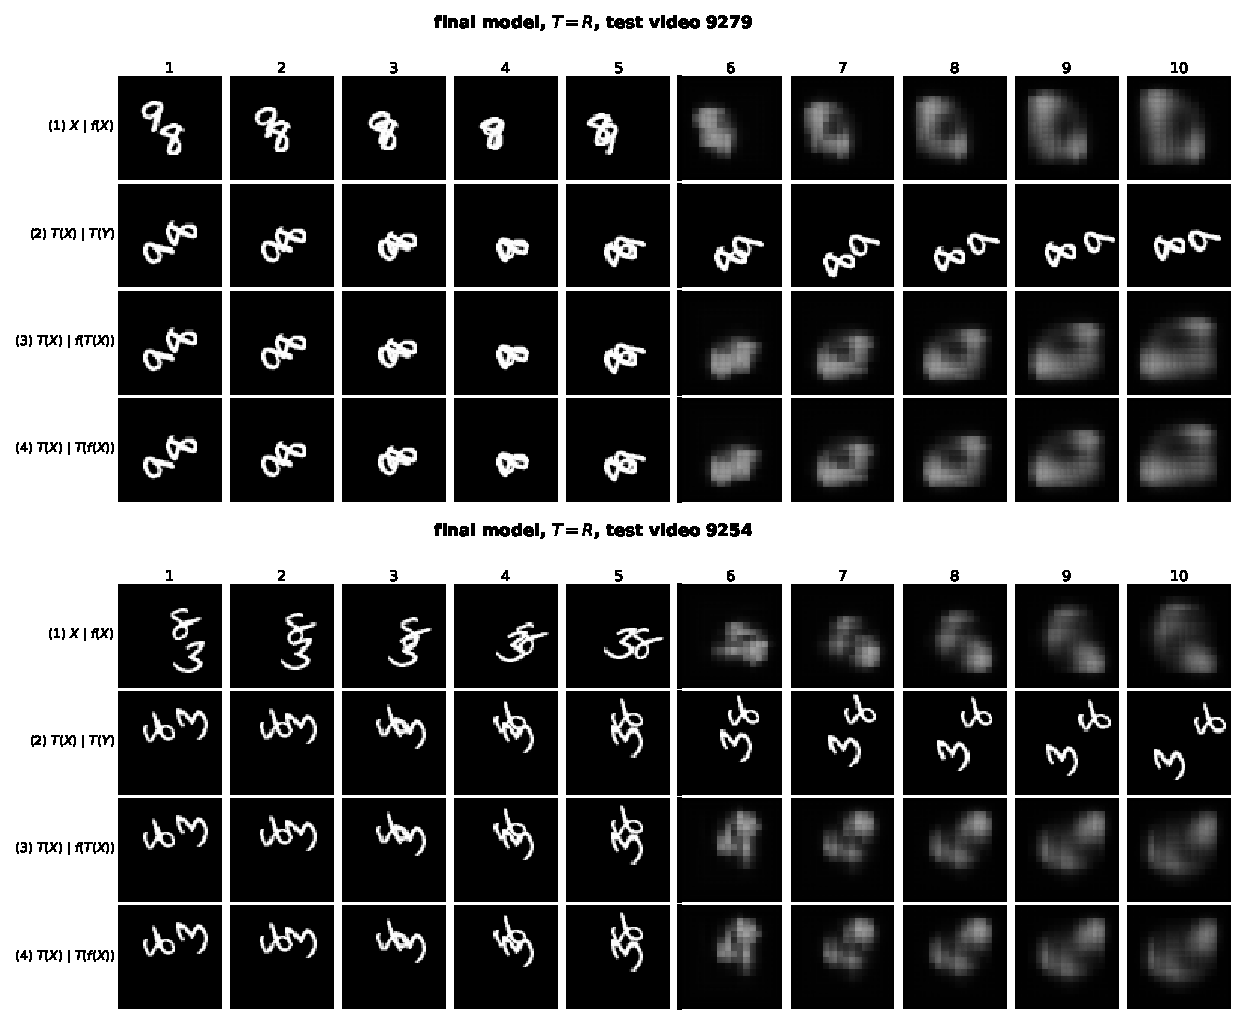
\includegraphics[width=0.88\linewidth]{fig6a_R.pdf}
\caption*{\textbf{Figure 6(a).} Figure 3 repeated with the final model (symmetrised D, seed 0) on exactly the same four test videos (top $T=M$: 9269, 9499; bottom $T=R$: 9279, 9254); rows as in Figure~\ref{fig:f3}. Rows 3 and 4 are identical by construction. GIFs: \texttt{figures/gifs/fig6a\_M\_rank1\_video9269.gif}, \texttt{fig6a\_M\_rank2\_video9499.gif}, \texttt{fig6a\_R\_rank1\_video9279.gif}, \texttt{fig6a\_R\_rank2\_video9254.gif}.}
\end{figure}
\begin{figure}[!htbp]\centering
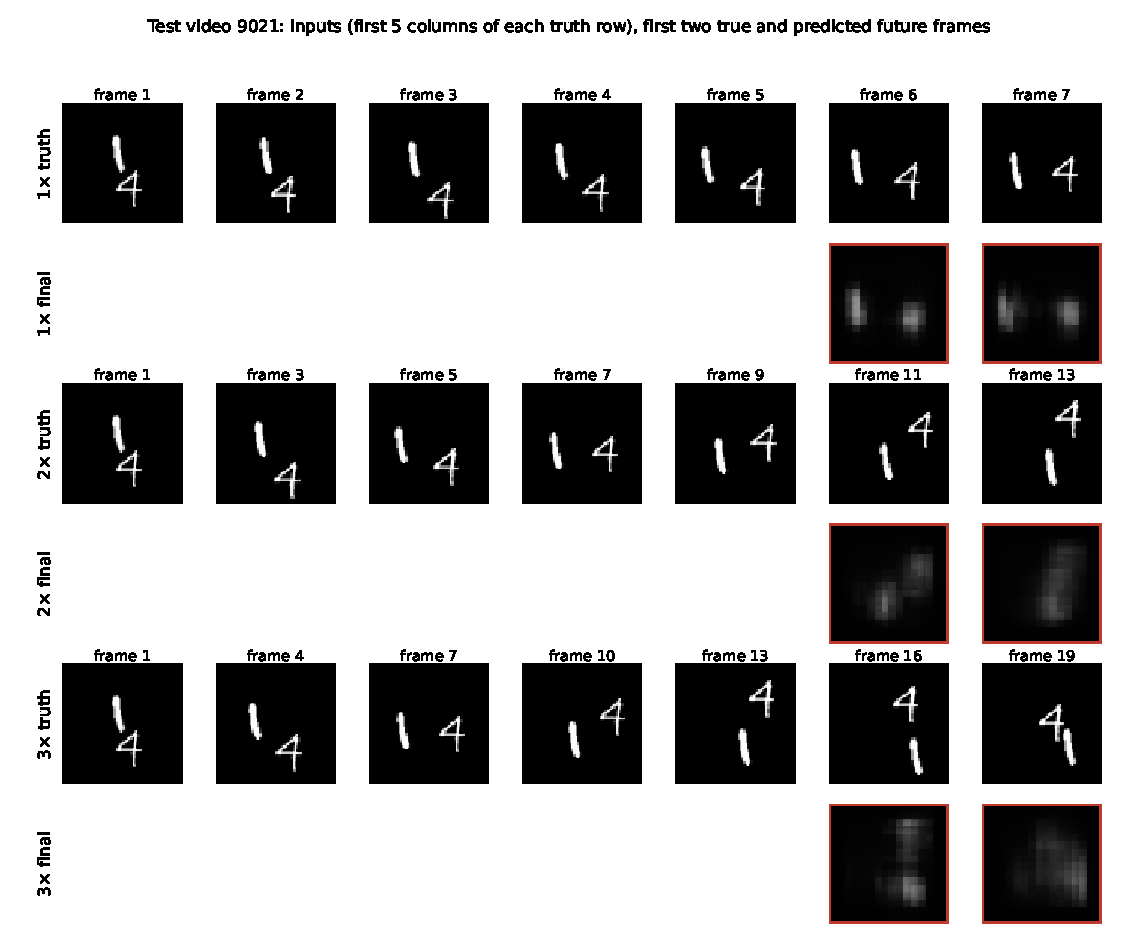
\includegraphics[width=0.93\linewidth]{fig6b_speed.pdf}
\caption*{\textbf{Figure 6(b).} Figure 5 repeated with the final model (symmetrised D, seed 0) on exactly the same test video (9021): inputs, first two true and predicted future frames at $1\times$, $2\times$, $3\times$.}\label{fig:f6b}
\end{figure}
\begin{table}[H]\centering\small
\caption*{\textbf{Table S1} (supplementary). Median centroid displacement (px) of a digit from the last input frame to the first forecast frame at $1\times$, $2\times$, $3\times$ (digits that form separate blobs in both frames; mean over seeds 0, 1 of each model's median; in brackets: median predicted/true per digit). Truth: 3.61, 7.07, 10.44 px.}
\begin{tabular}{lrrr}\toprule
Model & $1\times$ & $2\times$ & $3\times$ \\ \midrule
A (baseline) & 3.36 (96\%) & 2.49 (39\%) & 2.05 (22\%) \\
B (+sym.\ aug.) & 3.40 (97\%) & 2.64 (42\%) & 2.56 (27\%) \\
C (+speed aug.) & 3.23 (93\%) & 5.43 (84\%) & 6.84 (72\%) \\
D (reach 12 px) & 3.32 (96\%) & 5.73 (87\%) & 7.26 (77\%) \\
final: sym.\ D & 3.40 (97\%) & 5.80 (88\%) & 7.15 (76\%) \\
\bottomrule\end{tabular}\end{table}
\begin{table}[H]\centering\small
\caption*{\textbf{Table S2} (supplementary). $E^{(5)}$ (mean over seeds, $1\times$, $t=1$) on forward and on \emph{time-reversed} test videos, and on the 586 test videos whose digits overlap in frames 6--10 versus the other 414.}
\begin{tabular}{lrrrr}\toprule
Model & forward & time-reversed & overlap in 6--10 & no overlap \\ \midrule
A (baseline) & 0.0220 & 0.0219 & 0.0216 & 0.0225 \\
B (+sym.\ aug.) & 0.0223 & 0.0222 & 0.0219 & 0.0230 \\
C (+speed aug.) & 0.0269 & 0.0266 & 0.0259 & 0.0282 \\
D (reach 12 px) & 0.0267 & 0.0265 & 0.0257 & 0.0280 \\
final: sym.\ D & 0.0265 & 0.0264 & 0.0255 & 0.0280 \\
\bottomrule\end{tabular}\end{table}

\Q{Q2.15}{\textbf{Learned (B) versus built-in (symmetrised).} \emph{Consistency:} B reduces the gaps ($C_M$ $0.00177\to0.00128$, $C_R$ $0.00300\to0.00153$) but not to zero; the wrapped models have $C_M=C_R=0$ \emph{exactly}, for any $f$ (proof above). Augmentation only \emph{encourages} the symmetry on the data it saw; averaging \emph{imposes} it, so only the built-in version is exact. \emph{Accuracy on original clips ($1\times$):} sym.\ B $E^{(5)}=0.0217$ vs B $0.0223$ ($-2.8\%$); sym.\ D $0.0265$ vs D $0.0267$ ($-0.6\%$); on transformed clips, $E_M=E_R=E^{(5)}$ for the wrapped models by the identity above (B: $0.0223$/$0.0223$ vs $0.0223$). \emph{Inference cost:} B $0.57$\,s $\to$ sym.\ B $2.60$\,s ($4.5\times$) and D $0.65\to3.13$\,s ($4.8\times$) for 1000 videos (eight forward passes, not exactly $8\times$ because small batches do not saturate the GPU); training cost is unchanged for the wrapper, while B itself already costs $\approx1.6$--$1.7\times$ the training time per epoch. \textbf{When would built-in symmetry hurt?} Averaging eight predictions blurs when the predictions are sharp and the views disagree, i.e.\ when the world is \emph{not} symmetric: a drift or gravity in one direction, orientation-specific appearance that matters for the forecast, or a symmetry that holds only approximately. It did not hurt here: the dynamics (constant velocity, elastic bounces in a square box) are exactly $G$-symmetric and the forecasts are already blurry, so averaging acts like a small ensemble ($-0.6\%$ to $-2.8\%$ error).}

\Q{Q2.16}{\textbf{Video 9279, $T=R$ (Figures~\ref{fig:f3} and 6(a)).} Model A's two views disagreed (rotated input: stalled blob, centroid $0.27$\,px/frame vs truth $1.46$; original: $1.44$). In the final model the disagreement is gone: rows 3 and 4 are identical (centroid gap $0.0$\,px); but it is \emph{not} right: both views move at $0.79$\,px/frame (truth $1.46$), and the forecast's ink grows from $306$ to $480$ (truth $255\to273$), i.e.\ it still under-moves and blurs. Which change fixed what: \emph{symmetrisation} fixed the disagreement (consistency: $C_R=0$); \emph{symmetry augmentation (B)} reduced the stall in the rotated view ($0.27\to1.19$\,px/frame, B seed 0) --- so the stall was mostly appearance; \emph{speed augmentation and reach (C, D)} did not change this $1\times$ video ($D$: $0.78/1.11$, i.e.\ no improvement), and the remaining under-motion is the general $1\times$ cost of Q2.14 (D, C are less sharp at $1\times$ than A). In short: consistency repaired, accuracy on this overlap video not.}

\Q{Q2.17}{\textbf{Final verdict (150 words).} \emph{Partly.} Evidence for motion rather than memory: exact $G$-consistency ($C_M=C_R=0$, $E_M=E_R=E^{(5)}=0.0265$); the same error on \emph{time-reversed} videos ($0.0264$ vs $0.0265$, Table~S2); at $2\times$/$3\times$ the digits travel $88\%$/$76\%$ of the true distance (A: $39\%$/$22\%$) and $E^{(2)}$ falls to $0.0282$/$0.0318$ (A $0.0444$/$0.0516$). Against: forecasts stay blurry ($0.0265$, only $38\%$ below Blank) and under-move at $3\times$. \emph{A skeptic would be convinced} by sharp forecasts with the right displacement at speeds \emph{outside} the training set (e.g.\ non-integer or faster). \emph{Test not passed:} tracking digit identity through overlaps --- Figure~6a (video 9279) is still blurred and slow.}

% ============================================================== AI USE DISCLOSURE
\newpage
\section*{Generative-AI use disclosure (course AI policy)}
\addcontentsline{toc}{section}{Generative-AI use disclosure}

\noindent\textbf{Tool.} Cursor (Claude) in VS Code, used locally with the assignment folder and conda environment \texttt{PA1\_DL}.

\noindent\textbf{How it was used.} The assistant was used to understand the handout, to ask for section templates, and to sanity-check wording and numbers. Training, evaluation, file layout, and the submitted claims were the student's. Suggested text was kept only after it matched the handout and the saved result files.

\noindent\textbf{Prompts given by the student} (15 representative questions; not a request to complete the assignment):
\begin{enumerate}[leftmargin=*,itemsep=0.6pt]
\item ``Please explain Assignment~2 in your own words: what is Q1 vs Q2, and what must be in the report vs the GitHub repo?''
\item ``Give me a heading template for Question~1 that matches the PDF (architecture, assumptions, task, data, training, robustness). Do not fill the answers.''
\item ``Which river facts are given, and which ones am I allowed to assume? I want history length and the 60-minute horizon labelled as assumptions if the brief does not fix them.''
\item ``Is future rainfall allowed as an input? Is an already announced reservoir release allowed? Please quote the distinction.''
\item ``For Moving MNIST, may I use torchvision's built-in train/test split, or must I split by video index? I am using conda env \texttt{PA1\_DL}.''
\item ``What should Table~1 contain, and how are speed and the symmetry group $G$ defined in the handout? A checklist is enough.''
\item ``How do I count parameters of a ConvLSTM so I can check that Model~A is 480{,}784?''
\item ``What does the optical-flow figure need to show (inputs, arrows, calibration)? A caption template only.''
\item ``Give me a short markdown template for the Q2.5 prediction file. Remind me that it has to be committed before I run the mirror / rotation / speed tests.''
\item ``Same for Q2.11: a prediction template, and remind me it must be committed before I train B, C, and D.''
\item ``In the PDF, what is the difference between models A, B, C, and D? I will choose D myself; I only want the definitions.''
\item ``Write the symmetrised-forecaster formula from the handout so I can check my implementation of $C_T$ and $E_T$.''
\item ``Give me a report outline (Q1, Q2a, Q2b, tables, figures) with empty bullets. I will write the content.''
\item ``Please shorten my Question~1 headings and suggest how to draw the architecture in TikZ. Do not change the design.''
\item ``My GitHub URL is \url{https://github.com/ihuzafaone/DLSTG-PA2}, name Huzaifa, roll 25280009. Put those in the header only. Then list remaining PDF requirements I may have missed.''
\end{enumerate}

\noindent\textbf{Coding help (summary).} Asked for a repo layout, a Table~1 checklist, a parameter-count check for Model~A, a caption template for the optical-flow figure, a Q1 section template, a reminder of what Model~D is allowed to change, and a report outline. Did not ask the assistant to train models or to invent results.

\noindent\textbf{Help on code.} Example snippets and naming suggestions for data loading, ConvLSTM, metrics, training entry points, and symmetrisation (in this repo: \texttt{src/mmdata.py}, \texttt{src/models.py}, \texttt{src/evalkit.py}, \texttt{src/train.py}, \texttt{src/table1.py}, \texttt{src/fig1\_flow.py}, \texttt{q1/river\_prototype.py}). The student adapted those ideas, ran jobs in \texttt{PA1\_DL} on a local NVIDIA RTX~4060 Laptop GPU (8\,GB), and kept Model~D's dilation and the D$+$B run only after validation screening.

\noindent\textbf{My checks on code.} Confirmed Table~1 against the handout; confirmed Model~A (and the screened Model~D) at 480{,}784 parameters; confirmed that every reported test number matches the JSON files in \texttt{results/}.

\noindent\textbf{Question 1.} The assistant drafted empty six-heading templates and TikZ layout hints. History length $L{=}36$ and the six-step (60\,min) horizon are assumptions A1/A2 in the sense that the brief leaves both unspecified; the section keeps those separate from the given river. Future rain is not an input; an already announced release is. The diagram is the TikZ figure; headings were shortened by the student.

\noindent\textbf{Question 2.} The assistant explained required tables/figures and commented on scripts. The student ran Table~1, Figure~1, training, and evaluation, and checked the numbers. Q2.5 was written before the mirror, rotation, and speed tests; Q2.11 was written before training B, C, and D.

\noindent\textbf{Output kept from the assistant.} Clarifications of what the handout was asking, blank section templates, reminders of formulas already given in the brief, and help tightening wording, plus a checklist used on a final pass. Every number reported here was read off the student's own saved result files, never supplied by the assistant.

\end{document}
